\documentclass[a4paper]{article}
\usepackage{pgf,tikz,pgfplots}
\usetikzlibrary{arrows,decorations.markings}
\pgfplotsset{compat=1.15}
\usepackage{mathrsfs}
\usetikzlibrary{arrows}
%% Language and font encodings
\usepackage[english]{babel}
\usepackage[utf8x]{inputenc}
\usepackage[T1]{fontenc}
\usepackage{float}
%% Sets page size and margins
\usepackage[a4paper,top=3cm,bottom=2cm,left=3cm,right=3cm,marginparwidth=1.75cm]{geometry}
\usepackage{fancyhdr}
\pagestyle{fancy}
%% Useful packages
\usepackage{tensor}
\usepackage{xcolor}
\usepackage{color,soul}
\usepackage{amsmath}
\usepackage{amsthm}
\usepackage{enumitem}
\usepackage{eqnarray}
\usepackage{float}
\usepackage{esint}
\usepackage{wrapfig}
\usepackage{gensymb}
\usepackage{lipsum}
\usepackage{amssymb}
\usepackage{array}
\usepackage{tikz}
\usepackage[colorlinks=true, allcolors=blue]{hyperref}
\usepackage{graphicx}
\usepackage{amsmath}
\usepackage{amssymb}
\usepackage{graphicx}
\usepackage[colorlinks=true, allcolors=blue]{hyperref}
\usepackage{mathtools}
\DeclareMathOperator{\Proj}{Proj}
\DeclareMathOperator{\lcm}{lcm}
\DeclareMathOperator{\cosec}{cosec}
\DeclareMathOperator{\sgn}{sgn}
\DeclareMathOperator{\Span}{span}
\DeclareMathOperator{\nullity}{nullity}
\DeclarePairedDelimiter\floor{\lfloor}{\rfloor}
\DeclareMathOperator{\Res}{Res}
\DeclareMathOperator{\rank}{rank}
\DeclareMathOperator{\Ker}{Ker}
\DeclareMathOperator{\R}{R}
\DeclareMathOperator{\Tr}{Tr}
\DeclareMathOperator{\diag}{diag}
\DeclareMathOperator{\Log}{Log}
\DeclareMathOperator{\sech}{sech}
\DeclareMathOperator{\Var}{Var}
\newtheoremstyle{new2}% <name>
{2pt}% <Space above>
{2pt}% <Space below>
{\color{black}}% Body font
{}% <Indent amount>
{\bfseries\color{black}}% Theorem head font
{:}% <Punctuation after theorem head>
{.5em}% <Space after theorem headi>
{}% <Theorem head spec (can be left empty, meaning `normal')>
\theoremstyle{new2}
\newtheorem{ans}{Answer}[section]

\newcommand{\highlight}[1]{%
  \colorbox{red!50}{$\displaystyle#1$}}
  
\definecolor{darkblue}{RGB}{	0, 0, 139}
\newtheoremstyle{new}% <name>
{2pt}% <Space above>
{2pt}% <Space below>
{\color{darkblue}}% Body font
{}% <Indent amount>
{\bfseries\color{black}}% Theorem head font
{:}% <Punctuation after theorem head>
{.5em}% <Space after theorem headi>
{}% <Theorem head spec (can be left empty, meaning `normal')>
\theoremstyle{new}
\newtheorem{qns}{Problem}[section]
\setlength{\parindent}{0cm}
\title{\textbf{Part II REL Problem Sheet Solutions}}
\author{Tai Yingzhe, Tommy (ytt26)}
\date{}
\setlength{\parindent}{0cm}
\begin{document}
\maketitle
\tableofcontents
\subsection*{Acknowledgements:}
Many thanks to Sarah Williams for conducting the insightful example classes, and has thus contributed to my understanding of the course material.
\newpage
\section{Problem Sheet 1}
\subsection*{Special Relativity}
\begin{qns}[Spacetime interval]\leavevmode
\begin{enumerate}[label=(\alph*)]
\item Show that if two events are separated by a timelike interval, then there is a frame in which they occur at the same spatial location.
\item Similarly, if two events are separated by a spacelike interval, show there is a frame in which they are simultaneous.
\end{enumerate}
\end{qns}
\begin{ans}\leavevmode
\begin{enumerate}[label=(\alph*)]
\item Without loss of generality, align axes of $S$ such that $\Delta y=\Delta z=0$. Perform standard Lorentz boost to another frame $S'$:
$$\Delta y'=\Delta z'=0,\quad\Delta x'=\gamma(\Delta x-v\Delta t)$$
where we assumed frame $S'$ have velocity $0<|v/c|<1$. To ensure they occur at the same spatial location in frame $S'$:
$$\Delta x'=0\implies\frac{v}{c}=\frac{\Delta x}{c\Delta t}\implies|\Delta x|<c|\Delta t|$$
The spacetime interval is
$$\Delta s^2=(c\Delta t)^2-(\Delta x)^2-(\Delta y)^2-(\Delta z)^2=(c\Delta t)^2-(\Delta x)^2-0>0$$
and hence the events are time-like separated.
\item Again without loss of generality, $\Delta y=\Delta z=0$. Perform a standard Lorentz boost, i.e. $c\Delta t'=\gamma(c\Delta t-(v/c)\Delta x)$. For two events to be simultaneous in frame $S'$, $\Delta t'=0$, we have $$\frac{v}{c}=\frac{c\Delta t}{\Delta x}\implies\frac{\Delta t}{\Delta x}=\frac{v}{c^2}<1\implies c\Delta t<\Delta x$$
Again, assumed $0<|v/c|<1$ for frame $S'$. The spacetime interval is
$$\Delta s^2=(c\Delta t)^2-(\Delta x)^2-(\Delta y)^2-(\Delta z)^2=(c\Delta t)^2-(\Delta x)^2-0<0$$
and hence for such a frame $S'$, the events are space-like separated.
\end{enumerate}
\end{ans}
\begin{qns}[Spacetime interval]\leavevmode
\begin{enumerate}[label=(\alph*)]
\item Show that if an event A precedes an event B in some frame S at the same spatial location, then the event A precedes event B in all frames. 
\item Two general events A and B are separated in S by a spatial distance $\Delta r$. If event A causes event B, determine an inequality for the time difference between the events, $\Delta t=t_B-t_A$. Hence show that the events are causally related in all frames.
\end{enumerate}
\end{qns}
\begin{ans}\leavevmode
\begin{enumerate}[label=(\alph*)]
\item In frame $S$, if two events occur at the same spatial location $\Delta\mathbf{r}=\boldsymbol{0}$, then $\Delta t=t_B-t_A>0$, i.e. event A precedes event B. Under standard Lorentz boost,
$$c\Delta t'=\gamma(c\Delta t)>0$$
Hence $\Delta t'>0$ $\forall\gamma$, i.e. for all inertial frames related to $S$ by a Lorentz boost.
\item If A causes B, time is needed for a signal to propagate between them, i.e. $c|\Delta t|>|\Delta r|\implies\Delta s^2=(c\Delta t)^2-(\Delta r)^2>0$. The spatial separation along the Lorentz boost direction satisfy $\Delta x\leq\Delta r$. By invariance of the spacetime interval, we must have $|c\Delta t'|>|\Delta r'|$ in any frame. Choose axes in $S$ and $S'$ so in standard configuration,
$$\Delta x\leq\Delta r,~c\Delta t>\Delta r\implies c\Delta t'=\gamma(c\Delta t-v\Delta x)\implies c|\Delta t'|>|\Delta\mathbf{r}|$$
Hence, the two events are causally related in all frames.
\end{enumerate}
\end{ans}
\newpage
\begin{qns}[Spacetime diagram]\leavevmode
\begin{enumerate}[label=(\alph*)]
\item On a spacetime diagram with the $x$ and $ct$ axes of an inertial frame $S$ horizontal and vertical, respectively, construct the lines of constant $x'$ and $ct'$, where these coordinates refer to the frame $S'$ in standard configuration with $S$ (i.e., where $S'$ moves at a speed $v$ along the positive $x$-direction and the two frames coincide at $t = t' = 0$). Show that the angle between the $x$- and $x'$- axes is the same as that between the $ct$- and $ct'-$ axes and has the value $\tan^{-1}(v/c)$.
\item Sketch on your diagram the loci of events separated from the spacetime origin $x = ct = 0$ by a constant invariant interval $\Delta s^2=c^2t^2-x^2$ for positive (timelike) and negative (spacelike) values of $\Delta s^2$. How can these curves be used to calibrate lengths along the axes of the $S$ and $S'$ frames?
\item Use your diagram to illustrate graphically why a rod at rest in $S'$ is \textit{contracted} as measured in $S$, and the time on a clock at rest in $S'$ is \textit{dilated} as observed in $S$.
\end{enumerate}
\end{qns}
\begin{ans}\leavevmode
\begin{enumerate}[label=(\alph*)]
\item The $x'$ axis has equation $ct=vx/c$, while the $x$ axis is just a horizontal line. Simple trigonometry gives
$$\tan^{-1}(ct/x)=\tan^{-1}((vx/c)/x)=\tan^{-1}(\beta)$$
The $t'$ axis has equation $x=vt$, while the $t$ axis is just a vertical line. Simple trigonometry again gives
$$\tan^{-1}(x/ct)=\tan^{-1}(vt/ct)=\tan^{-1}(\beta)$$
\item The spacetime interval is $\Delta s^2=c^2t^2-x^2$ and are represented by hyperbolae. On the spacetime diagram below, we have $\Delta s^2<0$ (spacelike) and $\Delta s^2>0$ (timelike) to be represented by the red and blue curves respectively. The diagonal asymptotes are the worldlines of photons starting at the common spacetime origin, travelling at $\pm c$.
\begin{center}
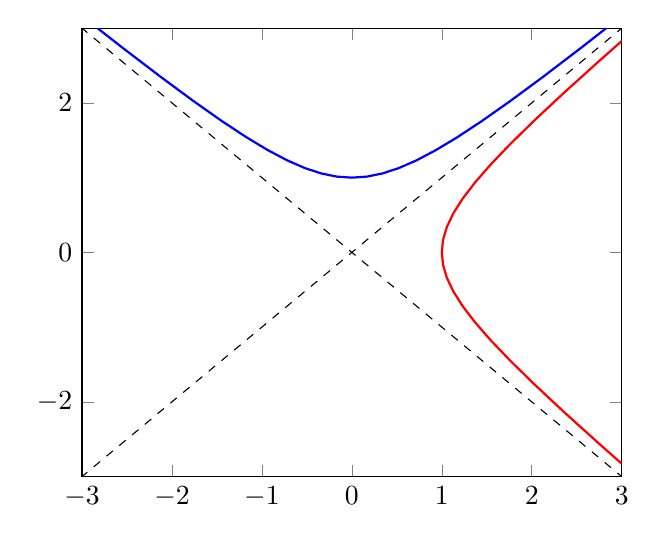
\begin{tikzpicture}
    \begin{axis}[
            xmin=-3,xmax=3,
        ymin=-3,ymax=3]
        \addplot [red,thick,domain=-2:2] ({cosh(x)}, {sinh(x)});
        \addplot [blue,thick,domain=-2:2] ({sinh(x)}, {cosh(x)});
        \addplot[black,dashed] expression {x};
        \addplot[black,dashed] expression {-x};
    \end{axis}
\end{tikzpicture}
\end{center}
The hyperbolae cross the $ct'$ and $x'$ axes at $ct'=\sqrt{\Delta s^2}$ (timelike) and at $x'=\sqrt{-\Delta s^2}$ (spacelike), allowing us to calibrate the spacetime axes in different frames. As a consistency check, the gradient of either hyperbolae is
$$2ct\frac{d(ct)}{dx}-2x=0\implies\frac{d(ct)}{dx}=\frac{x}{ct}$$
The gradient of the spacelike hyperbolae, at $ct'=0$, is $\beta$, same as the gradient of the $ct'$ axis (with equation $ct=\frac{v}{c}x$). Similarly, the gradient of the timelike hyperbolae, at $x'=0$, is $\beta^{-1}$, same as the gradient of the $x'$ axis (with equation $x=\frac{v}{c}ct$).
\item The fact that the spacetime interval hyperbolic curves can be used to calibrate lengths along the axes of the $S$ and $S'$ frames, we can demonstrate length contraction and time dilation. 
\begin{itemize}
    \item Time dilation: Suppose we have a clock with worldline $x'=0$ $\forall t'$ which measures a period $ct'=cT_0$. Let this event have spacetime coordinates ($ct_A'=cT_0$, $x_A'=0$), i.e. lie on the $ct'$ axis (with equation $ct_A\beta=x_A$). The spacetime interval curve $\Delta s^2=c^2T_0^2$ connects points on the $ct'$- and $ct$-axes with length $cT_0$. 
    $$c^2T_0^2=\Delta s^2=c^2t_A^2-x_A^2=c^2t_A^2(1-\beta^2)\implies T_0^2=\frac{t_A^2}{\gamma^2}$$
    To measure the period in $S$, we need to measure the time between two marked events at the same place. We can see that the time elapsed in frame $S$, $t_A$ is longer than the time elapsed in the clock's own rest frame $T_0$.
    \item Length contraction: Suppose we have a rod of length $\ell_0$ at rest in frame $S'$. Let the point corresponding to the end of the rod be event B of spacetime coordinates $(x_B'=\ell_0,t_B'=0)$, i.e. lie on the $x'$ axis (with equation $ct_B=\beta x_B)$. Again, the hyperbola (of space-like interval) connects points on the $x'$ and $x$-axes with length $\ell_0$.
    $$-\ell_0^2=\Delta s^2=c^2t_B^2-x_B^2=\beta^2x_B^2-x_B^2\implies x_B'^2=\gamma^2x_B^2$$
    To measure the length of the rod $\Delta x$ in $S$, we need to mark out the positions of both ends simultaneously. We can see the length measured in the frame $S$, $x_B$, is smaller than its rest length $\ell_0$.
\end{itemize}
\end{enumerate}
\end{ans}
\begin{qns}[Lorentz boost]
An inertial frame $S'$ is related to the frame $S$ by a boost of $\vec{v}$ whose components in $S$ are $(v_x, v_y, v_z)$. Show that the coordinates $(ct', x', y', z')$ and $(ct, x, y, z)$ of an event are related by
$$\begin{pmatrix}ct'\\x'\\y'\\z'\\\end{pmatrix}=\begin{pmatrix}\gamma&-\gamma\beta_x&-\gamma\beta_y&-\gamma\beta_z\\-\gamma\beta_x&1+\alpha\beta_x^2&\alpha\beta_x\beta_y&\alpha\beta_x\beta_z\\-\gamma\beta_y&\alpha\beta_y\beta_x&1+\alpha\beta_y^2&\alpha\beta_y\beta_z\\-\gamma\beta_z&\alpha\beta_z\beta_x&\alpha\beta_z\beta_y&1+\alpha\beta_z^2\\\end{pmatrix}\begin{pmatrix}ct\\x\\y\\z\\\end{pmatrix}$$
where $\vec{\beta}=\vec{v}/c$, $\gamma=(1-|\vec{\beta}|^2)^{-1/2}$ and $\alpha=(\gamma-1)/|\vec{\beta}|^2$. (Hint: resolve the 3-vector position with components $(x, y, z)$ into parallel and perpendicular parts with respect to $\vec{\beta}$, and similarly in the $S'$ frame.)
\end{qns}
\begin{ans}
Resolve $\vec{r}=(x,y,z)$ into parallel and perpendicular parts with respect to $\vec{\beta}$:
$$\vec{r}=\vec{r}_\parallel+\vec{r}_\perp=\frac{(\vec{r}\cdot\vec{\beta})\vec{\beta}}{|\vec{\beta}|^2}+\bigg(\vec{r}-\frac{(\vec{r}\cdot\vec{\beta})\vec{\beta}}{|\vec{\beta}|^2}\bigg)$$
Similarly, we can resolve $\vec{r'}$. Only the component parallel to the Lorentz boost is transformed:
$$\vec{r'}\cdot\hat{\vec{\beta}}=\gamma(\vec{r}\cdot\hat{\vec{\beta}}-\beta ct)\implies\vec{r'}_\parallel=\frac{\vec{r'}\cdot\vec{\beta}}{|\vec{\beta}|}\hat{\vec{\beta}}=\hat{\vec{\beta}}\gamma(\vec{r}\cdot\hat{\vec{\beta}}-\beta ct)$$
The perpendicular components remain unchanged:
$$\vec{r'}_\perp=\vec{r'}-(\vec{r'}\cdot\hat{\vec{\beta}})\hat{\vec{\beta}}=\vec{r}-(\vec{r}\cdot\hat{\vec{\beta}})\hat{\vec{\beta}}$$
We then have
\begin{align}
    \vec{r'}&=\vec{r'}_\parallel+\vec{r'}_\perp\nonumber\\&=-\gamma\beta ct\vec{\hat{\beta}}+\vec{r}+(\vec{r}\cdot\vec{\beta})\vec{\beta}\alpha\nonumber\\&=-\gamma\beta \hat{\vec{\beta}}ct+\begin{pmatrix}1+\alpha\beta_x^2&\alpha\beta_x\beta_y&\alpha\beta_x\beta_z\\\alpha\beta_y\beta_x&1+\alpha\beta_y^2&\alpha\beta_y\beta_z\\\alpha\beta_z\beta_x&\alpha\beta_z\beta_y&1+\alpha\beta_z^2\\\end{pmatrix}\vec{r}\nonumber
\end{align}
where $\alpha=\frac{\gamma-1}{|\vec{\beta}|^2}$ and $(r_i\beta_i)\beta_j=r_i(\beta_i\beta_j)$, noting that $\beta_i\beta_j$ is a matrix. Now, the time coordinate transforms like
$$ct'=\gamma(ct-\vec{r}\cdot\vec{\beta})$$
This gives the first row of the desired matrix.
\end{ans}
\newpage
\begin{qns}[Velocity composition]
In a given inertial frame, two particles are shot out simultaneously from a given
point, with equal speeds v in orthogonal directions. What is the speed of each particle
relative to the other?
\end{qns}
\begin{ans}
Let particle A and B have velocities $v(0,1,0)$ and $v(1,0,0)$ respectively. In the frame of particle B (Lorentz boost by $v(1,0,0)$), particle B observes particle A to have $u_x=0$, $u_y=v$, $u_z=0$ and so by usual velocity transformation,
$$u_x'=-v,\quad u_y'=v/\gamma_v,\quad u_z'=0$$
The relative speed is then $v(1+\gamma_v^{-2})^{1/2}=v(2-(v/c)^2)^{-1/2}$. We could have also worked in the frame of particle A.
\end{ans}
\begin{qns}[Velocity composition]\leavevmode
\begin{enumerate}[label=(\alph*)]
\item Frame $S'$ moves with speed $v$ relative to frame $S$ in standard configuration. A rod at rest in frame $S'$ makes an angle $\theta'$ with respect to the forward direction of motion. What is the angle $\theta$ measured in S?
\item If a bullet is fired in $S'$ at speed $u'$ at an angle $\theta'$ with respect to the forward direction of motion, what is the angle $\theta$ measured in $S$? What if the bullet is a photon?
\end{enumerate}
\end{qns}
\begin{ans}\leavevmode
\begin{enumerate}[label=(\alph*)]
\item Let the two ends of the rod (with proper length $\ell_0$) be A and B where A is at the origin of $\mathbb{R}^3$. In frame $S'$, the spacetime coordinates of A and B are $(ct',0,0,0)$ and $(ct',\ell_0\cos\theta',\ell_0\sin\theta',0)$ respectively. Inverse Lorentz transform back to frame $S$, the coordinates for A and B in frame $S$ are respectively
$$\begin{pmatrix}\gamma ct'\\\gamma\beta ct'\\0\\0\\\end{pmatrix}=\begin{pmatrix}ct\\\beta ct=vt\\0\\0\\\end{pmatrix},\quad\begin{pmatrix}\gamma ct'+\gamma\beta\ell_0\cos\theta'\\\gamma\ell_0\cos\theta'+\gamma\beta ct'\\\ell_0\sin\theta'\\0\\\end{pmatrix}=\begin{pmatrix}ct\\\gamma\ell_0\cos\theta'+\beta(ct-\gamma\beta\ell_0\cos\theta')=\ell_0\gamma^{-1}\cos\theta'+vt\\\ell_0\sin\theta'\\0\\\end{pmatrix}$$
where the time coordinate in frame $S$ has to be $ct$. The back and the front both moves at speed $v$, as expected. The angle in frame $S$ thus satisfy
$$\tan\theta=\frac{\ell_0\sin\theta'}{\ell_0\cos\theta'/\gamma}=\gamma\tan\theta'$$
\item Inverse transform the velocity components for $u'$:
$$u_x=\frac{u'\cos\theta'+v}{1+(u'v/c^2)\cos\theta'},\quad u_y=\frac{u'\sin\theta'}{\gamma_v(1+(u'v/c^2)\cos\theta')},\quad u_z=0$$
The angle $\theta$ in $S$ satisfies
$$\tan\theta=\frac{u_y}{u_x}=\frac{u'\sin\theta'}{\gamma_v(u'\cos\theta'+v)}$$
If the object was a photon, then $u=c$ and we recover the light aberration relation
$$\tan\theta=\frac{\sin\theta'}{\gamma_v(\cos\theta'+\beta)}$$
\end{enumerate}
\end{ans}
\newpage
\begin{qns}[Aberration]
Frame $S'$ moves with speed $v$ relative to frame $S$ in standard configuration. Neutral $\pi$-mesons at rest in $S'$ decay into two photons that are emitted isotropically. Show that the angular distribution of photons in $S$ is
$$P(\theta)d\theta=\frac{\sin\theta d\theta}{2\gamma^2(1-\beta\cos\theta)^2}$$
\end{qns}
\begin{ans}
From Q6, we have 
$$\cos\theta'=\frac{\cos\theta-\beta}{1-\beta\cos\theta}\implies\frac{d\cos\theta'}{d\cos\theta}=\frac{1-\beta\cos\theta-(\cos\theta-\beta)(-\beta)}{(1-\beta\cos\theta)^2}=\frac{1}{\gamma^2(1-\beta\cos\theta)^2}$$
Since photons are emitted isotropically in $S'$, we have $P(\theta',\phi')=\frac{1}{4\pi}$. Then integrate over $\phi$:
$$P(\theta')d\theta'=\int_0^{2\pi}P(\theta',\phi')\sin\theta'd\theta'd\phi'=\frac{1}{2}\sin\theta'd\theta'$$
The number of photons emitted in either frame is the same, i.e. $P(\theta)d\theta=P(\theta')d\theta'$.
$$\implies P(\theta)=P(\theta')\frac{d\theta'}{d\theta}=\frac{1}{2}\sin\theta'\frac{d\theta'}{d\theta}=-\frac{1}{2}\frac{d(\cos\theta')}{d\theta}=-\frac{1}{2}\frac{d(\cos\theta')}{d\cos\theta}\frac{d\cos\theta}{d\theta}=\frac{\sin\theta}{2\gamma^2(1-\beta\cos\theta)^2}$$
i.e. the photons are strongly `beamed' in the $x$-direction due to aberration.
\end{ans}
\begin{qns}[Rectilinear acceleration]\leavevmode
\begin{enumerate}[label=(\alph*)]
\item A spaceship travels in a straight line at a variable speed $u(t)$ in some inertial frame $S$. An observer on the spaceship measures his acceleration to be $f(\tau)$, where $\tau$ is his proper time. If at $\tau=0$ the spaceship has a speed $u_0$ in $S$ show that
$$\frac{u(\tau)-u_0}{1-u(\tau)u_0/c^2}=c\tanh\psi(\tau)$$
where $c\psi(\tau)=\int_0^\tau f(\tau')d\tau'$. Show that the speed of the spaceship can never reach $c$.
\item If the spaceship left base at time $t=\tau=0$ and travelled forever in a straight line with constant acceleration $g$ (for comfort), how long by the spaceship clock does it take to reach a star 10 light years from the base?
\end{enumerate}
\end{qns}
\begin{ans}\leavevmode
\begin{enumerate}[label=(\alph*)]
\item $f(\tau)$ is the acceleration in the instantaneous rest frame (IRF). At proper time $\tau$, the speed is $u$ and increases by $f(\tau)d\tau$ in the IRF. In $S$, the speed increases by $du$. By velocity addition,
$$u+du=\frac{fd\tau+u}{1+(u/c^2)fd\tau}=u\bigg(1-\frac{u}{c^2}fd\tau\bigg)+fd\tau+\dots=u+\frac{fd\tau}{\gamma_u^2}+\dots\implies\frac{du}{d\tau}=\frac{f}{\gamma_u^2}$$
Let $u/c=\tanh\theta(\tau)$, then
$$\frac{du}{d\tau}=\frac{c}{\cosh^2\theta}\frac{d\theta}{d\tau}\implies\frac{d\theta(\tau)}{d\tau}=\frac{f(\tau)}{c}$$
since $\gamma_u=\frac{1}{\sqrt{1-u^2}}=\frac{1}{\sqrt{1-\tanh^2\theta(\tau)}}=\cosh\theta$ (definition of rapidity). We then have
$$c\theta(\tau)-c\tanh^{-1}(u_0/c)=\int_0^\tau f(\tau')d\tau'$$
where the integration constant occur since $u=u_0$ at $\tau=0$. Evaluate $\tanh\psi(\tau)$:
$$\tanh\psi=\tanh(\theta-\tanh^{-1}(u_0/c))=\frac{\tanh\theta-u_0/c}{1-(u_0/c)\tanh\theta}=\frac{1}{c}\frac{u-u_0}{1-uu_0/c^2}$$
where $\psi(\tau)=\frac{1}{c}\int_0^\tau f(\tau')d\tau'=\theta(\tau)-\tanh^{-1}(u_0/c)$. Upon rearranging, we have
$$\frac{u}{c}=\frac{(u_0/c)+\tanh\psi}{1+(u_0/c)\tanh\psi}$$
For $0\leq\psi<\infty$, the RHS increases monotonically from $u_0/c$ to 1, i.e. $u(\tau)$ approaches but never exceeds $c$.
\begin{center}
\begin{tikzpicture}
      \draw[->] (0,0) -- (6,0) node[right] {$\psi$};
      \draw[->] (0,0) -- (0,2) node[left] {$u/c$};
      \draw[domain=0:6,smooth,variable=\x,blue] plot ({\x},{(0.5+tanh(\x))/(1+0.5*tanh(\x))});
      \draw (0,0) node[left]{0};
      \draw (0,0.5) node[left]{$u_0/c$};
      \draw (0,1) node[left]{1};
    \end{tikzpicture}
\end{center}
Alternatively, we may Lorentz transform the acceleration directly. In the instantaneous rest frame at $\tau$, $u'(\tau)=0$ and $\frac{du'}{dt'}=\frac{du'}{d\tau}=f(\tau)$. Transforming back to the frame $S$, we have
$$\frac{du}{dt}=\frac{\frac{du'(\tau)}{d\tau}}{\gamma_u^3(1-0)^3}=\bigg(1-\frac{u^2}{c^2}\bigg)^{3/2}f(\tau)\implies\frac{du}{d\tau}=\bigg(1-\frac{u^2}{c^2}\bigg)f(\tau)$$
$$\implies c^2\bigg[\frac{1}{c}\tanh^{-1}(u/c)\bigg]^{u(\tau)}_{u_0}=\int^\tau_0f(\tau')d\tau'\implies\tanh^{-1}(u(\tau)/c)-\tanh^{-1}(u_0/c)=\frac{1}{c}\int_0^\tau f(\tau')d\tau'$$
Let the RHS $\frac{1}{c}\int_0^\tau f(\tau')d\tau'$ be $\psi(\tau)$, then again by angle addition, we evaluate $\tanh\psi(\tau)$ to obtain our result.
\item By definition of proper time,
$$c^2d\tau^2=c^2dt^2-dx^2=c^2dt^2(1-u^2/c^2)$$
We have $d\tau/dt=1/\gamma_u=1/\cosh\psi$, so since
$$c\tanh\psi=u=\frac{dx}{d\tau}\frac{d\tau}{dt}\implies\frac{dx}{d\tau}=c\sinh\psi$$
But $\psi(\tau)=(g/c)\int_0^\tau d\tau=g\tau/c$, so
$$x-0=\frac{c^2}{g}\bigg[\cosh(g\tau'/c)\bigg]^{\tau}_0=\frac{c^2}{g}[\cosh(g\tau/c)-1]$$
where the integration constant is obtained from $x(\tau=0)=0$. We have $x=10$ light years and so
$$xg/c^2=\frac{(365.25)(24)(3600)(10)(9.81)}{3\times10^8}=10.32$$
and hence $g\tau/c=\cosh^{-1}(10.32+1)=3.118$. Finally,
$$\tau=\frac{3.118}{9.81}\frac{3\times10^8}{24(3600)(365.25)}=3.02\text{ years}$$
\end{enumerate}
\end{ans}
\newpage
\subsection*{Manifolds and Coordinates}
\begin{qns}[Metric tensor, volume coordinate]
In 3D Euclidean space, coordinates $x'^a$ are related to Cartesian coordinates $x^a$ by
$$x^1=x'^1+x'^2,\quad  x^2=x'^1-x'^2,\quad x^3=2x'^1x'^2+x'^3$$
Describe the coordinate surfaces in the primed system. Obtain the metric functions $g_{ab}'$ in the primed system and hence show that these coordinates are not orthogonal. Calculate the volume element $dV$ in the primed coordinate system.
\end{qns}
\begin{ans}
To describe the surfaces associated to the primed coordinates, we rearrange to get
$$x'^1=0.5(x^1+x^2),\quad x'^2=0.5(x^1-x^2),\quad x'^3=x^3-0.5((x^1)^2-(x^2)^2)$$
$x'^1=\text{const.}$ and $x'^2=\text{const.}$ are diagonal planes in the $x$-space, while $x'^3=\text{const.}$ are hyperbolic paraboloids with principal axes along $x^1$ and $x^2$ directions. The spacetime invariant is
\begin{align}
    ds^2&=(dx^1)^2+(dx^2)^2+(dx^3)^2\nonumber\\&=(dx'^1+dx'^2)^2+(dx'^1-dx'^2)^2+(2x'^1dx'^2+2x'^2dx'^1+dx'^3)^2\nonumber\\&=2(dx'^1)^2+2(dx'^2)^2+4(x'^1)^2(dx'^2)^2+4(x'^2)^2(dx'^1)^2+(dx'^3)^2\nonumber\\&~~ +8x'^1x'^2~dx'^1~dx'^2+4x'^1~dx'^2~dx'^3+4x'^2~dx'^1~dx'^3\nonumber\\&=2(1+2(x'^2)^2)(dx'^1)^2+2(1+2(x'^1)^2)(dx'^2)^2+8x'^1x'^2~dx'^1~dx'^2+4x'^1~dx'^2~dx'^3+4x'^2~dx'^1~dx'^3+(dx'^3)^2\nonumber
\end{align}
with the metric tensor as
$$g'_{ab}=\begin{pmatrix}2(1+2(x'^2)^2)&4x'^1x'^2&2x'^2\\4x'^1x'^2&2(1+2(x'^1)^2)&2x'^1\\2x'^2&2x'^1&1\\\end{pmatrix}$$
Since the metric tensor is not diagonal, it is not an orthogonal coordinate system. The determinant and hence the volume element in the primed coordinate system is 
\begin{align}
    &\det g'\nonumber\\&=2(1+2(x'^2)^2)[2(1+2(x'^1)^2-4(x'^1)^2]-4(x'^1)(x'^2)[4x'^1~x'^2-4x'^1~x'^2]+2x'^2[8(x'^1)^2(x'^2)-4(x'^2)(1+2(x'^1)^2)]\nonumber\\&=4\implies dV'=\sqrt{\det g'}dx'^1~dx'^2~dx'^3=2dx'^1~dx'^2~dx'^3\nonumber
\end{align}
\end{ans}
\begin{qns}[Line element, volume]
Show that the line element of a 3-sphere of radius $a$ embedded in 4D Euclidean space can be written in the form
$$ds^2=a^2[d\chi^2+\sin^2\chi(d\theta^2+\sin^2\theta d\phi^2)]$$
Hence, in this 3D non-Euclidean space, calculate the area of the 2-sphere defined by $\chi=\chi_0$. Also find the total volume of the 3D space.
\end{qns}
\begin{ans}
The 3-sphere $x^2+y^2+z^2+w^2=a^2$ is parametrized by
$$w=a\cos\chi,\quad x=a\sin\chi\sin\theta\cos\phi,\quad y=a\sin\chi\sin\theta\sin\phi,\quad z=a\sin\chi\cos\theta,\quad 0\leq\chi\leq\pi$$
where $\theta,\phi$ are the usual spherical polar coordinates. The infinitesimal elements are
$$dw=-a\sin\chi d\chi,\quad dx=a\cos\chi\sin\theta\cos\phi d\chi+a\sin\chi d(\sin\theta\cos\phi)$$
$$dy=a\cos\chi\sin\theta\sin\phi d\chi+a\sin\chi d(\sin\theta\sin\phi),\quad dz=a\cos\chi\cos\theta d\chi+a\sin\chi d\cos\theta$$
The interval is
\begin{align}
    ds^2&=dw^2+dx^2+dy^2+dz^2\nonumber\\&=a^2\sin^2\chi d\chi^2+a^2\cos^2\chi d\chi^2+a^2\sin^2\chi(d\theta^2+\sin^2\theta d\phi^2)+2a^2\sin\chi\cos\chi d\chi[\sin\theta\cos\phi d(\sin\theta\cos\phi)\nonumber\\&~~+\sin\theta\sin\phi d(\sin\theta\sin\phi)+\cos\theta d\cos\theta]\nonumber\\&=a^2d\chi^2+a^2\sin^2\chi(d\theta^2+\sin^2\theta d\phi^2)\nonumber
\end{align}
On the 2-sphere $\chi=\chi_0$, the induced line element is
$$ds^2=a^2\sin^2\chi_0(d\theta^2+\sin^2\theta d\phi^2)$$
as expected. The 2-volume and 3-volume respectively are
$$dV_{(2)}=a^2\sin^2\chi_0\sin\theta~d\theta~d\phi\implies V_{(2)}=4\pi a^2\sin^2\chi_0,\quad dV_{(3)}=a^3\sin^2\chi\sin\theta~d\chi~d\theta~d\phi\implies V_{(3)}=2\pi^2a^3$$
\end{ans}


\newpage
\section{Problem Sheet 2}
\subsection*{Vector and Tensor Algebra}
\begin{qns}[Metric tensor, dual basis]
In 3D Euclidean space, coordinates $x'^a$ are related to Cartesian coordinates $x^a$ by
$$x^1=x'^1+x'^2,\quad  x^2=x'^1-x'^2,\quad x^3=2x'^1x'^2+x'^3$$
\begin{enumerate}[label=(\alph*)]
\item Express the coordinate basis vectors $\mathbf{e_a'}=\frac{\partial}{\partial x'^a}$ for the primed coordinates in terms of those for the Cartesian coordinates. How are these related to the intersections of the coordinate surfaces that you sketched in Question 9 of Examples Sheet 1? By considering $\mathbf{g}(\mathbf{e_a'},\mathbf{e_b'})$ obtain the components of the metric $g'_{ab}$. (Hint: since the original coordinates are Cartesian, $\mathbf{g}(\mathbf{e_a},\mathbf{e_b})=\delta_{ab}$.) 
\item Let the vector $\mathbf{v}=\mathbf{e_1}$. Write down the components $v^a$ and those of the associated dual vector $v_a$. Calculate the components of the same vector $\mathbf{v}$ and its associated dual vector in the primed coordinates. 
\end{enumerate}
\end{qns}
\begin{ans}\leavevmode
\begin{enumerate}[label=(\alph*)]
\item Using chain rule,
$$e_1'=\frac{\partial x^1}{\partial x'^1}\frac{\partial}{\partial x^1}+\frac{\partial x^2}{\partial x'^1}\frac{\partial}{\partial x^2}+\frac{\partial x^3}{\partial x'^1}\frac{\partial}{\partial x^3}=\frac{\partial}{\partial x^1}+\frac{\partial}{\partial x^2}+2x'^2\frac{\partial}{\partial x^3}=e_1+e_2+(x^1-x^2)e_3$$
$$e_2'=\frac{\partial x^1}{\partial x'^2}\frac{\partial}{\partial x^1}+\frac{\partial x^2}{\partial x'^2}\frac{\partial}{\partial x^2}+\frac{\partial x^3}{\partial x'^2}\frac{\partial}{\partial x^3}=\frac{\partial}{\partial x^1}-\frac{\partial}{\partial x^2}+2x'^1\frac{\partial}{\partial x^3}=e_1-e_2+(x^1+x^2)e_3$$
$$e_3'=\frac{\partial x^1}{\partial x'^3}\frac{\partial}{\partial x^1}+\frac{\partial x^2}{\partial x'^3}\frac{\partial}{\partial x^2}+\frac{\partial x^3}{\partial x'^3}\frac{\partial}{\partial x^3}=e_3$$
$e_3'=e_3$ is the derivative with respect to $x'^3$ at fixed $x'^1$ and $x'^2$, so along the directions of the line of intersection at constant $x'^1$ and $x'^2$. We have the metric tensor to be 
$$g(e_a',e_b')=g_{ab}'=\frac{\partial x^c}{\partial x'^a}\frac{\partial x^d}{\partial x'^b}g_{cd}$$
$$g_{11}'=g_{11}+g_{22}+g_{33}(2x'^2)^2=2+4(x'^2)^2,\quad g_{22}'=2+4(x'^2)^2$$
$$g_{12}'=g_{11}\frac{\partial x^1}{\partial x'^1}\frac{\partial x^1}{\partial x'^2}+g_{22}\frac{\partial x^2}{\partial x'^1}\frac{\partial x^2}{\partial x'^2}+g_{33}\frac{\partial x^3}{\partial x'^1}\frac{\partial x^3}{\partial x'^2}=1-1+2x'^22x'^1=4x'^1x'^2=g_{21}'$$
$$g_{13}'=g_{11}\frac{\partial x^1}{\partial x'^1}\frac{\partial x^1}{\partial x'^3}+g_{22}\frac{\partial x^2}{\partial x'^1}\frac{\partial x^2}{\partial x'^3}+g_{33}\frac{\partial x^3}{\partial x'^1}\frac{\partial x^3}{\partial x'^3}=2x'^2=g_{31}'$$
$$g_{33}'=g_{11}\frac{\partial x^1}{\partial x'^3}\frac{\partial x^1}{\partial x'^3}+g_{22}\frac{\partial x^2}{\partial x'^3}\frac{\partial x^2}{\partial x'^3}+g_{33}\frac{\partial x^3}{\partial x'^3}\frac{\partial x^3}{\partial x'^3}=1$$
where we get the same result as that in Q9 of the previous example sheet.
\item The vector is $v=v^ae_a\implies v^a=\tensor*{\delta}{*_{}^{a}_{1}}=(1,0,0)^T$. The dual vector is
$$v_b=g_{ab}v^a=\delta_{ab}\tensor*{\delta}{*_{}^{a}_{1}}=\delta_{b1}=(1,0,0)$$
where $g_{ab}=\delta_{ab}$ in the coordinate basis and it is used to lower the index. Now in the primed coordinates,
$$v'^a=\frac{\partial x'^a}{\partial x^b}v^b=\frac{\partial x'^a}{\partial x^1}=\begin{pmatrix}1/2\\1/2\\-(x'^1+x'^2)\\\end{pmatrix}$$
where $x'^1=0.5(x^1+x^2)$, $x'^2=0.5(x^1-x^2)$ and $x'^3=x^3-2x'^1x'^2=x^3-0.5((x^1)^2+(x^2)^2)$. Similarly,
$$v_a'=\frac{\partial x^b}{\partial x'^a}v_b=\frac{\partial x^1}{\partial x'^a}=(1,1,0)$$
\end{enumerate}
\end{ans}
\newpage
\subsection*{Vector and tensor calculus on manifolds}
\begin{qns}[Tensor]\leavevmode
\begin{enumerate}[label=(\alph*)]
\item If the tensor $A_{ab}$ is an antisymmetric tensor, $S_{ab}$ is a symmetric tensor and $T_{ab}$ is a general tensor, show that $A^{ab}T_{ab} = A^{ab}T_{[ab]}$ and $S^{ab}T_{ab}=S^{ab}T_{(ab)}$. 
\item If $v_a$ are the components of a dual vector, show that in an arbitrary coordinate system $A_{ab} = \partial_bv_a−\partial_av_b$ are the components of a type-(0, 2) tensor. Show further, for a general antisymmetric tensor $A_{ab}$, that $B_{abc} = \partial_cA_{ab} + \partial_aA_{bc} + \partial_bA_{ca}$ are the components of a type-(0, 3) tensor. What are the symmetry properties of $B_{abc}$?
\end{enumerate}
\end{qns}
\begin{ans}\leavevmode
\begin{enumerate}[label=(\alph*)]
\item We are given $A_{ab}=-A_{ba}$ and $S_{ab}=S_{ba}$, so
$$A^{ab}T_{[a,b]}=\frac{1}{2}A^{ab}(T_{ab}-T_{ba})=\frac{1}{2}(A^{ab}T_{ab}+A^{ab}T_{ab})=A^{ab}T_{ab}$$
where $A^{ba}T_{ba}=A^{ab}T_{ab}$. Similarly,
$$S^{ab}T_{(a,b)}=\frac{1}{2}S^{ab}(T_{ab}+T_{ba})=S^{ab}T_{ab}$$
\item The covariant derivative of a dual vector is given as
$$\nabla_bv_a=\partial_bv_a-\Gamma^c_{ba}v_c\implies \nabla_bv_a-\nabla_av_b=\partial_bv_a-\Gamma_{ba}^cv_c-\partial_av_b+\Gamma_{ab}^cv_c=\partial_bv_a-\partial_av_a=A_{ab}$$
where the connection is torsion free in GR, i.e. $\Gamma_{ba}^c=\Gamma^c_{ab}$. LHS is a tensor so $A_{ab}$ is also a tensor and it is of type (0,2). Now, the covariant derivative for a general antisymmetric tensor $A_{ab}$ is
$$\nabla_cA_{ab}=\partial_cA_{ab}-\Gamma_{ca}^dA_{db}-\Gamma_{cb}^dA_{ad}$$
Do permutations of the indices to get two other equations. Add all three up and we have
\begin{align}
&=\nabla_cA_{ab}+\nabla_aA_{bc}+\nabla_bA_{ca}\nonumber\\&=\partial_cA_{ab}+\partial_aA_{bc}+\partial_bA_{ca}-\Gamma_{ca}^d(A_{db}+A_{bd})-\Gamma^d_{cb}(A_{ad}+A_{da})-\Gamma^d_{ab}(A_{dc}+A_{cd})\nonumber\\&=\partial_cA_{ab}+\partial_aA_{bc}+\partial_bA_{ca}+0\nonumber\\&=B_{abc}\nonumber
\end{align}
where $A$ is anti-symmetric and the connection $\Gamma_{ab}^c$ is symmetric in the bottom indices $a,b$. The LHS is a tensor, so $B_{abc}$ is also a tensor, i.e. type (0,3) tensor. Notice that $B_{abc}$ is symmetric for any even permutations of $(a,b,c)$. Now, anti-symmetrize completely:
$$B_{[a,b,c]}=\frac{1}{6}(B_{abc}+B_{bca}+B_{cab}-B_{bac}-B_{acb}-B_{cba})=\frac{1}{2}(B_{abc}-B_{acb})$$
Since $A$ is anti-symmetric, it follows that
$$B_{acb}=\partial_bA_{ac}+\partial_aA_{cb}+\partial_cA_{ba}=-\partial_bA_{ca}-\partial_aA_{bc}-\partial_cA_{ab}=-B_{abc}$$
i.e. $B_{abc}$ is anti-symmetric in the indices $c$ and $b$. Hence, we must have $B_{abc}$ to be totally anti-symmetric, i.e. $B_{[a,b,c]}=\frac{1}{2}(B_{abc}+B_{abc})=B_{abc}$.
\end{enumerate}
\end{ans}
\newpage
\begin{qns}[Metric connection]\leavevmode
\begin{enumerate}[label=(\alph*)]
\item  If $g = \det(g_{ab})$ is the determinant of the metric, show that $\partial_cg = gg^{ab}(\partial_cg_{ab})$.
\item Verify directly, in a general coordinate system, that $\nabla_cg_{ab} = 0$ for the covariant derivative constructed with the metric connection.
\item For a diagonal metric $g_{ab}$, show
that the connection coefficients are given by (with $a\neq b\neq c$ and no summation over
repeated indices)
\end{enumerate}
$$\Gamma_{bc}^a=0,\quad\Gamma_{aa}^b=-\frac{1}{2g_{bb}}\frac{\partial g_{aa}}{\partial x^b},\quad\Gamma_{ba}^a=\Gamma_{ab}^a=\frac{\partial}{\partial x_b}(\ln\sqrt{|g_{aa}|})$$
\end{qns}
\begin{ans}\leavevmode
\begin{enumerate}[label=(\alph*)]
\item We have $g=\det g_{ab}\implies\ln \det g_{ab}=\Tr(\ln g_{ab})$, so
$$\frac{1}{g}\partial_cg=\Tr(g^{-1}\partial_cg)\implies\frac{1}{g}\partial_cg=g^{ab}\partial_cg_{ab}$$
where we used definition of trace.
\item The covariant derivative of the metric tensor is
$$\nabla_cg_{ab}=\partial_cg_{ab}-\Gamma_{ca}^dg_{db}-\Gamma_{cb}^dg_{ad}$$
where the metric connection is
$$\Gamma_{bc}^a=\frac{1}{2}g^{ad}(\partial_bg_{cd}+\partial_cg_{db}-\partial_dg_{bc})$$
Hence,
\begin{align}
    \nabla_cg_{ab}&=\partial_cg_{ab}-\frac{1}{2}g_{db}g^{d\rho}(\partial_cg_{a\rho}+\partial_ag_{\rho c}-\partial_\rho g_{ca})-g_{ad}\frac{1}{2}g^{d\rho}(\partial_cg_{b\rho}+\partial_bg_{\rho c}-\partial_\rho g_{cb})    \nonumber\\&=\partial_cg_{ab}-\frac{1}{2}(\partial_cg_{ab}+\partial_ag_{bc}-\partial_bg_{ca})-\frac{1}{2}(\partial_cg_{ba}+\partial_bg_{ac}-\partial_ag_{cb})\nonumber\\&=0\nonumber
\end{align}
\item Now, $g_{ab}$ is diagonal.
$$\Gamma_{bc}^a=\frac{1}{2}g^{ad}(\partial_bg_{cd}+\partial_cg_{db}-\partial_dg_{bc})=0$$
if $a\neq b\neq c$, all the $\partial g$ terms are zero since $g$ is diagonal tensor. If two indices are the same, we contract:
$$\Gamma_{bb}^a=\frac{1}{2}g^{ad}(\partial_bg_{bd}+\partial_bg_{db}-\partial_dg_{bb})=-\frac{1}{2}g^{aa}\partial_ag_{bb}=-\frac{1}{2g_{aa}}\frac{\partial g_{bb}}{\partial x^a}$$
$$\Gamma_{ba}^a=\frac{1}{2}g^{ad}(\partial_bg_{ad}+\partial_ag_{db}-\partial_dg_{ba})=\frac{1}{2}g^{aa}(\partial_bg_{aa})=\frac{1}{2g_{aa}}\frac{\partial g_{aa}}{\partial x^b}=\frac{\partial}{\partial x^b}\ln\sqrt{|g_{aa}|}$$
where we bear in mind $g$ is diagonal.
\end{enumerate}
\end{ans}
\newpage
\begin{qns}[Connection]
In 2D Euclidean space, the line element in plane-polar coordinates is
$$ds^2=d\rho^2+\rho^2d\phi^2$$
\begin{enumerate}[label=(\alph*)]
\item Obtain the non-zero connection coefficients
$$\Gamma_{\rho\phi}^\phi=\Gamma_{\phi\rho}^\phi=1/\rho,\quad\Gamma_{\phi\phi}^\rho=-\rho$$
\item If the coordinate components $v^a$ of a vector $\mathbf{v}$ are written as $v^\rho$ and $v^\rho$, show that the divergence of $\mathbf{v}$ is
$$\nabla_av^a=\frac{1}{\rho}\frac{\partial}{\partial\rho}(\rho v^\rho)+\frac{\partial v^\phi}{\partial\phi}$$
What would be the equivalent result in terms of the components of $\mathbf{v}$ in an orthonormal basis aligned with the coordinate directions?
\item Show that the Laplacian of a scalar field $f$ is
$$\nabla^2f=\frac{1}{\rho}\frac{\partial}{\partial\rho}\bigg(\rho\frac{\partial f}{\partial\rho}\bigg)+\frac{1}{\rho^2}\frac{\partial^2f}{\partial\phi^2}$$
\end{enumerate}
\end{qns}
\begin{ans}\leavevmode
\begin{enumerate}[label=(\alph*)]
\item From the line element, we have $g_{\rho\rho}=1$ and $g_{\phi\phi}=\rho^2$. From Q3, 
$$\Gamma_{\rho\phi}^\phi=\frac{\partial}{\partial\rho}\ln\sqrt{|g_{\phi\phi}|}=\frac{\partial\ln\rho}{\partial\rho}=\frac{1}{\rho}=\Gamma_{\phi\rho}^\phi,\quad\Gamma_{\phi\phi}^\rho=-\frac{1}{2g_{\rho\rho}}\frac{\partial g_{\phi\phi}}{\partial\rho}=-\frac{2\rho}{2}=-\rho$$
\item The covariant derivative is
\begin{align}
    \nabla_av^a&=\partial_av^a+\Gamma_{ab}^av^b\nonumber\\&=\partial_\rho v^\rho+\partial_\phi v^\phi+\Gamma_{a\rho}^av^\rho+\Gamma_{a\phi}^a v^\phi\nonumber\\&=\partial_\rho v^\rho+\partial_\phi v^\phi+(\Gamma_{\rho\rho}^\rho+\Gamma_{\phi\rho}^\phi)v^\rho+(\Gamma_{\rho\phi}^\rho+\Gamma_{\phi\phi}^\phi) v^\phi\nonumber\\&=\partial_\rho v^\rho+\partial_\phi v^\phi+\frac{1}{\rho}v^\rho\nonumber\\&=\frac{1}{\rho}\partial_\rho(\rho v^\rho)+\partial_\phi v^\phi\nonumber
\end{align}
Set $\boldsymbol{e_\rho}=\frac{\partial}{\partial\rho}$, $\boldsymbol{e_\phi}=\frac{\partial}{\partial\phi}$, it follows that the unit vectors are
$$\boldsymbol{\hat{e}_a}=\frac{1}{\sqrt{g_{aa}}}\boldsymbol{e_a}\implies\boldsymbol{\hat{e}_\rho}=\boldsymbol{e_\rho},~\boldsymbol{\hat{e}_\phi}=\frac{1}{\rho}\boldsymbol{e_\phi}$$
So written in terms of the unit vectors
$$\mathbf{v}=v^\rho\boldsymbol{e_\rho}+v^\phi\boldsymbol{e_\phi}=v^{\hat{\rho}}\boldsymbol{\hat{e}_\rho}+\frac{v^{\hat{\phi}}}{\rho}\boldsymbol{\hat{e}_\phi}\implies v^{\hat{\rho}}=v^\rho,~\frac{v^{\hat{\phi}}}{\rho}=v^\phi$$
Hence, the divergence, in an orthonormal basis, is given as
$$\nabla_av^a=\frac{1}{\rho}\partial_\rho(\rho v^{\hat{\rho}})+\frac{1}{\rho}\partial_\phi(v^{\hat{\phi}})$$
\item The Laplacian is $\nabla^2f=\nabla_a\nabla^af$ but $\nabla^af=g^{ab}\partial_bf$. The gradient is
$$\nabla^af=(g^{\rho\rho}\partial_\rho f,g^{\phi\phi}\partial_\phi f)=(\partial_\rho f,\rho^{-2}\partial_\phi f)$$
The Laplacian is then obtained from the divergence result in (a):
$$\nabla^2f=\frac{1}{\rho}\partial_\rho(\rho\partial_\rho f)+\partial_\phi(\rho^{-2}\partial_\phi f)=\frac{1}{\rho}\frac{\partial}{\partial\rho}\bigg(\rho\frac{\partial f}{\partial\rho}\bigg)+\frac{1}{\rho^2}\frac{\partial^2f}{\partial\phi^2}$$
\end{enumerate}
\end{ans}
\newpage
\begin{qns}[Geodesic, Parallel transport]
On the surface of a unit sphere $ds^2 = d\theta^2 + \sin^2\theta d\phi^2$.
\begin{enumerate}[label=(\alph*)]
\item  Calculate the connection coefficients in the $(\theta,\phi)$ coordinate system directly from the metric.
\item By considering the ‘Lagrangian’ $L=g_{ab}\dot{x}^a\dot{x}^b$, derive the equations for an affinely-parameterised geodesic on the surface of a sphere in the coordinates $(\theta, \phi)$ and thereby verify your answer to (a). Hence show that, of all the circles of constant latitude on a sphere, only the equator is a geodesic.
\item A vector $\mathbf{v}$ of unit length is defined at the point $(\theta_0,0)$ and is parallel to the circle $\phi = 0$. Calculate the components of $\mathbf{v}$ after it has been parallel transported around the circle $\theta=\theta_0$. Hence show that, in general, after parallel transport, the direction of $\mathbf{v}$ is different, but its length is unchanged.
\end{enumerate}
\end{qns}
\begin{ans}\leavevmode
\begin{enumerate}[label=(\alph*)]
\item Reading off from $ds^2$, we have $g_{\theta\theta}=1$ and $g_{\phi\phi}=\sin^2\theta$, which is a diagonal metric. The connection coefficients are
$$\Gamma_{\phi\phi}^\theta=-\frac{1}{2g_{\theta\theta}}\partial_\theta g_{\phi\phi}=-\sin\theta\cos\theta,\quad\Gamma_{\theta\phi}^\theta=\frac{1}{2g_{\theta\theta}}\partial_\phi g_{\theta\theta}=0$$
$$\Gamma^{\phi}_{\theta\theta}=-\frac{1}{2g_{\phi\phi}}\partial_\phi g_{\theta\theta}=0,\quad\Gamma_{\phi\theta}^\phi=\frac{1}{2g_{\phi\phi}}\partial_\theta g_{\phi\phi}=\frac{2\sin\theta\cos\theta}{2\sin^2\theta}=2\cot\theta$$
\item The Lagrangian is
$$L=g_{ab}\dot{x}^a\dot{x}^b=g_{\theta\theta}\dot{x}^\theta\dot{x}^\theta+g_{\phi\phi}\dot{x}^\phi\dot{x}^\phi$$
The Euler-Lagrange equations (and hence the equations of motion) are
$$0=\frac{d}{d\lambda}\frac{\partial L}{\partial\dot{\theta}}-\frac{\partial L}{\partial\theta}=\frac{d}{d\lambda}2\dot{\theta}-2\sin\theta\cos\theta\dot{\phi}^2\implies\ddot{\theta}=\sin\theta\cos\theta\dot{\phi}^2$$
$$0=\frac{d}{d\lambda}\frac{\partial L}{\partial\dot{\phi}}-\frac{\partial L}{\partial\phi}=\frac{d}{d\lambda}2\sin^2\theta\dot{\phi}-0=4\sin\theta\cos\theta\dot{\theta}\dot{\phi}+2\sin^2\theta\ddot{\phi}\implies\ddot{\phi}+2\cot\theta\dot{\theta}\dot{\phi}=0$$
Compare to the geodesic equation $\ddot{x}^a+\Gamma^a_{bc}\dot{x}^b\dot{x}^c=0$:
$$\ddot{\theta}+\Gamma_{\phi\phi}^\theta\dot{\phi}\dot{\phi}+\Gamma_{\theta\phi}^\theta\dot{\theta}\dot{\phi}=\ddot{\theta}-\sin\theta\cos\theta\dot{\phi}^2+0=0$$
$$\ddot{\phi}+\Gamma_{\theta\theta}^\phi\dot{\theta}\dot{\theta}+\Gamma_{\phi\theta}^\phi\dot{\theta}\dot{\phi}=\ddot{\phi}+2\cot\theta\dot{\theta}\dot{\phi}+0=0$$
which recover the two equations of motion. The great circles of constant latitude have constant $\theta$. These great circles are geodesics and must satisfy the equation of motion:
$$0=\ddot{\theta}=\sin\theta\cos\theta\dot{\phi}^2\implies\sin\theta\cos\theta=0\implies\theta=\pi/2$$
which is the equator.
\item For a vector to be parallel transported, it must satisfy
$$\dot{v}^a+\Gamma_{bc}^av^b\dot{x}^c=0$$
Choosing the affine parameter to be $\phi$, we then have a pair of coupled first order ODE:
$$\frac{dv^\theta}{d\lambda}+\Gamma_{\phi\phi}^\theta v^\phi\frac{d\phi}{d\lambda}=0\implies\frac{dv^\theta}{d\phi}=\sin\theta_0\cos\theta_0 v^\phi,\quad \frac{dv^\phi}{d\lambda}+\Gamma_{\theta\phi}^\phi v^\theta\frac{d\phi}{d\lambda}=0\implies\frac{dv^\phi}{d\phi}=-\cot\theta_0 v^\theta$$
Hence we must have
$$\frac{d^2v^\theta}{d\phi^2}=\sin\theta_0\cos\theta_0(-\cot\theta_0)v^\theta=-\cos^2\theta_0v^\theta\implies v^\theta(\phi)=c_1\cos(\phi\cos\theta_0)+c_2\sin(\phi\cos\theta_0)$$
To find $v^\phi$,
$$v^\phi\sin\theta_0\cos\theta_0=-c_1\cos\theta_0\sin(\phi\cos\theta_0)+\cos\theta_0 c_2\cos(\phi\cos\theta_0)\implies v^\phi(\phi)=\frac{-c_1\sin(\phi\cos\theta_0)+c_2\cos(\phi\cos\theta_0))}{\sin\theta_0}$$
The initial norm of the vector is 1:
$$1=g_{ab}v^a(0)v^b(0)=|c_1|^2+\sin^2\theta_0\frac{|c_2|^2}{\sin^2\theta_0}=|c_1|^2+|c_2|^2$$
To find the initial direction of $v^a$:
$$v^a(0)=|v||e^a|\cos\chi$$
where $\chi$ is the relative angle between $v$ and the coordinate basis vector $e^a$. We have
$$v^\theta(0)=\cos\alpha,\quad v^\phi(0)=\frac{1}{\sin\theta_0}\cos(\pi/2-\alpha)=\frac{\sin\alpha}{\sin\theta_0}\implies c_1=\cos\alpha,~c_2=\sin\alpha$$
where $|e^\theta|=1$, $|e^\phi|=\frac{1}{\sin\theta_0}$. The coefficients $c_1,c_2$ do ensure the initial norm is 1. The norm after parallel transport is
\begin{align}
&g_{ab}v^a(2\pi)v^b(2\pi)\nonumber\\&=(\cos\alpha\cos(\phi\cos\theta_0))+\sin\alpha\sin(\phi\cos\theta_0))^2+\frac{(-\cos\alpha\sin(\phi\cos\theta_0)+\sin^2\theta_0\sin\alpha\cos(\phi\cos\theta_0))^2}{\sin^2\theta_0}\nonumber\\&=\cos^2(\alpha-\phi\cos\theta_0)+\frac{\sin^2(\alpha-\phi\cos\theta_0)}{\sin^2\theta_0}\sin^2\theta_0\nonumber\\&=1=g_{ab}v^a(0)v^b(0)\nonumber
\end{align}
which is unchanged by parallel transport. The direction of the vector after parallel transport is
\begin{align}
    g_{ab}v^a(0)v^b(2\pi)&=\cos\alpha\cos(\alpha-2\pi\cos\theta_0)+\sin\alpha\sin(\alpha-2\pi\cos\theta_0)\nonumber\\&=\cos(\alpha-(\alpha-2\pi\cos\theta_0))\nonumber\\&=\cos(2\pi\cos\theta_0)\nonumber
\end{align}
This verifies the general result that after parallel transport, the norm of a vector is unchanged but the direction does changes. In this case, the direction does not change only if $\theta_0=\pi/2$.
\end{enumerate}
\end{ans}
\begin{qns}[Geodesic]
A hypersurface $\mathcal{H}$ within a manifold $\mathcal{M}$ contains a non-null curve $\mathcal{C}$. Give a geometric argument showing that if $\mathcal{C}$ is a geodesic in $\mathcal{M}$, it is also a geodesic in $\mathcal{H}$. Give an example to show that the converse is not necessarily true.
\end{qns}
\begin{ans}
If $\mathcal{C}$ lies in $\mathcal{H}$, and it is extremal in $\mathcal{M}$, it must also be extremal for the subset of variations that lie in $\mathcal{H}$, hence it is a geodesic in $\mathcal{H}$. The converse is not true. The great circle connecting north and south poles on a 2-sphere is not a geodesic in $\mathbb{R}^3$.
\end{ans}
\newpage
\begin{qns}[Optional]
A surface $\mathcal{H}$ of $M$ dimensions is embedded in ND Euclidean space ($N > M$). The surface is specified in terms of coordinates $u^I$ ($I =1,\dots, M$) in the surface by the $N$ functions $x^a(u)$, where $x^a$ are Cartesian coordinates in the embedding space.
\begin{enumerate}[label=(\alph*)]
\item Show, by considering $ds^2=\delta_{ab}dx^adx^b$, that the metric induced on $\mathcal{H}$ is given 
$$g_{IJ}=\delta_{ab}\frac{\partial x^a}{\partial u^I}\frac{\partial x^b}{\partial u^J}$$
where implicit summation over repeated indices should be assumed throughout.
\item Show that the metric connection on $\mathcal{H}$ satisfies
$$g_{IL}\Gamma^L_{JK}=\delta_{ab}\frac{\partial x^a}{\partial u^I}\frac{\partial^2x^b}{\partial u^J\partial u^K}$$
\item A vector $\mathbf{A}$ lies in the tangent space to $\mathcal{H}$ at some point P. By considering the relation between coordinate basis vectors $\partial/\partial u^I$ in $\mathcal{H}$ and those in the embedding space, $\partial/\partial x^a$, show that the coordinate components $A^I$ and $A^a$ are related by
$$A^a=A^I\frac{\partial x^a}{\partial u^I}\bigg|_P$$
\item  A neighbouring point Q in $\mathcal{H}$ is displaced from P by infinitesimal coordinate differentials $\delta u^I$. A vector $\mathbf{A}_{\parallel}$ is defined in the tangent space to $\mathcal{H}$ at Q by displacing the vector $\mathbf{A}$ from P to Q in the embedding space, keeping its components $A^a$ fixed, and then taking the projection into the surface at $Q$. Show that
$$A^I(P)\frac{\partial x^a}{\partial u^I}\bigg|_P=A_{\parallel}^I(Q)\frac{\partial x^a}{\partial u^I}\bigg|_Q+A^a_\perp(Q)$$
where $A^a_\perp(Q)$ are the Cartesian components of the projection of the displaced vector normal to the surface at $Q$, so that
$$\delta_{ab}A_\perp^a(Q)\frac{\partial x^b}{\partial u^I}\bigg|_Q=0$$
By writing $A^I_\parallel(Q)=A^I(P)+\delta A^I$, and expanding the $(\partial x^a/\partial u^I)_Q$ about the point P, show that to first-order in small quantities
$$g_{IK}(P)\delta A^K=-\delta_{ab}\frac{\partial x^a}{\partial u^I}\bigg|_P\frac{\partial^2x^b}{\partial u^J\partial u^K}\bigg|_PA^K(P)\delta u^J$$
Hence show that the change $\delta A^K$ is the same as would be obtained by parallel transporting in the surface from P to Q: $\delta A^K=-\Gamma^K_{JL}(P)A^L(P)\delta u^J$. (This question shows that infinitesimal parallel transport in the curved surface is equivalent to parallel transport in the Euclidean embedding space followed by projection into the surface.)
\end{enumerate}
\end{qns}
\begin{ans}\leavevmode
\begin{enumerate}[label=(\alph*)]
\item The metric in Euclidean space and in $\mathcal{H}$ are respectively
$$ds^2=\delta_{ab}dx^adx^b=\delta_{ab}\frac{\partial x^a}{\partial u^I}\frac{\partial x^b}{\partial u^J}du^Idu^J,\quad ds^2=g_{IJ}du^Idu^J$$
Comparing them gives the desired result, i.e. $g_{IJ}=\delta_{ab}\partial_Ix^a\partial_Jx^b$. From now on, we will notate $\partial/\partial u^I$ as $\partial_I$.
\item The metric connection satisfies
\begin{align}
    g_{IL}\Gamma^L_{JK}&=\frac{1}{2}g_{IL}g^{LM}(\partial_Jg_{MK}+\partial_Kg_{MJ}-\partial_Mg_{JK})\nonumber\\&=\frac{1}{2}\tensor*{\delta}{*_{}^{M}_{I}}(\partial_Jg_{MK}+\partial_Kg_{MJ}-\partial_Mg_{JK})\nonumber\\&=\frac{1}{2}(\partial_Jg_{IK}+\partial_Kg_{IJ}-\partial_Ig_{JK})\nonumber\\&=\frac{1}{2}(\partial_J\delta_{ab}\partial_Ix^a\partial_Kx^b+\partial_K\delta_{ab}\partial_Ix^a\partial_Jx^b-\partial_I\delta_{ab}\partial_Jx^a\partial_Kx^b)\nonumber\\&=\frac{1}{2}\delta_{ab}[(\partial_Ix^a)(\partial_J\partial_Kx^b)+(\partial_Jx^a)(\partial_K\partial_Ix^b)]=\delta_{ab}(\partial_Ix^a)(\partial_J\partial_Kx^b)\nonumber
\end{align}
where $\delta_{ab}$ is symmetric and we used result from part (a).
\item Consider a vector $A\in\mathcal{T}_P(\mathcal{H})$,
$$A=A^I\frac{\partial}{\partial u^I}\bigg|_P=A^I\frac{\partial x^a}{\partial u^I}\frac{\partial}{\partial x^a}$$
Since the basis is $\partial_a$, it thus has components $A^a=A^I\partial_Ix^a|_P$.
\item At P, the components is $A^I(P)\partial_Ix^a|_P$. At a neighbouring point $Q$, the displaced vector is (upon taking the projection at $Q$)
$$A_Q=A^I(P)\partial_Ix^a|_P\frac{\partial}{\partial u}\bigg|_Q$$
This can be written as a superposition of
\begin{itemize}
    \item a component in the tangent space $A_\parallel^I(Q)\partial_Ix^a|_Q\frac{\partial}{\partial x^a}|_Q$;
    \item a component normal to the surface $A^a_\perp\frac{\partial}{\partial x^a}|_Q$.
\end{itemize}
Let $B\in\mathcal{T}_Q(\mathcal{H})$, then $B$ has the form
$$B=B^I\partial_I|_Q=B^I\partial_Ix^a|_Q\frac{\partial}{\partial x^a}\bigg|_Q$$
where $B^I\partial_Ix^a|_Q$ is the component in the embedding space. If $A^a_\perp\frac{\partial}{\partial x^a}|_Q$ is perpendicular to the tangent space, then for any vector $B$ in the tangent space,
$$0=A_\perp\cdot B=\delta_{ab}A^a_\perp B^I\partial_Ix^b|_Q\implies \delta_{ab}A^a_\perp\partial_Ix^b|_Q=0$$
since the result is true $\forall B\in\mathcal{T}_Q(\mathcal{H})$. Contract the component of $A_Q$ with $\delta_{ab}\partial_Jx^b|_Q$ to single out the component in the tangent space:
\begin{equation}
\delta_{ab}\partial_Jx^b|_QA^I(P)\partial_Ix^a|_P=\delta_{ab}\partial_Jx^b|_QA^I_\parallel(Q)\partial_Ix^a|_Q=A_{\parallel}^I(Q)g_{IJ}(Q)\label{**}
\end{equation}
where we used the result from part (a). If $A_\parallel^I(Q)=A^I(P)+\delta A^I$ and using $g_{IJ}(Q)\approx g_{IJ}(P)+\delta u^K\partial_Kg_{IJ}|_P$ , then keeping to first order of infinitesimal changes, the RHS of Eqn.(**) gives
$$A^I(P)\bigg[g_{IJ}(P)+\delta u^K~\partial_Kg_{IJ}|_P+\dots\bigg]+\delta A^I(g_{IJ}(P)+\dots)$$
whereas using $\partial_Ix^a|_Q\approx\partial_Ix^a|_P+\partial_I\partial_Kx^a|_P\delta u^K$, the LHS of (**) gives
$$\delta_{ab}A^I(P)\partial_Ix^a|_P\bigg[\partial_Jx^b|_P+\partial_J\partial_Kx^b|_P\delta u^K+\dots\bigg]=A^I(P)g_{IJ}(P)+A^I(P)\delta_{ab}\partial_Ix^a|_P\partial_J\partial_Kx^b|_P\delta u^K$$
Rearranging gives
\begin{align}
    \delta A^Ig_{IJ}(P)&=-A^I(P)(\partial_Kg_{IJ}|_P-\delta_{ab}\partial_Ix^a|_P\partial_J\partial_Kx^b|_P)\delta u^K\nonumber\\&=-\delta_{ab}A^I(P)[\partial_K(\partial_Ix^a\partial_Jx^b)-(\partial_Ix^a)(\partial_J\partial_Kx^b)]|_P\delta u^K\nonumber\\&=-\delta_{ab}A^I(P)(\partial_I\partial_Kx^a)|_P(\partial_Jx^b)|_P\delta u^K\nonumber
\end{align}
where we used result from part a. Relabelling indices gives
\begin{align}
g_{IK}(P)\delta A^K&=-\delta_{ab}\partial_Ix^a|_P\partial_J\partial_Kx^b|_PA^K(P)\delta u^J\nonumber\\&=-g_{IL}(P)\Gamma^L_{JK}(P)A^K(P)\delta u^J\nonumber\\&=-g_{IK}(P)\Gamma^K_{JL}(P)A^L(P)\delta u^J\nonumber\\\implies \delta A^K&=-\Gamma^K_{JL}A^L\delta u^J\nonumber
\end{align}
i.e. the infinitesimal parallel transport in a curved surface is equivalent to parallel transport in the Euclidean embedding space, followed by a projection onto the surface.
\end{enumerate}
\end{ans}

\newpage
\subsection*{Minkowski spacetime}
\begin{qns}[Photon, null path]
In Minkowski spacetime, two uniformly-moving observers $\mathcal{E}$ and $\mathcal{R}$ have 4-velocities $u$ and $v$, respectively.
\begin{enumerate}[label=(\alph*)]
\item  Show that $u^\mu v_\mu=c^2\gamma_V$, where $V$ is their relative speed.
\item  If $\mathcal{E}$ emits a photon that is subsequently received by $\mathcal{R}$, show that the ratio of the emitted and received photon frequencies is given by
$$\frac{v_{\mathcal{E}}}{v_{\mathcal{R}}}=\frac{u^\mu p_\mu}{v^\nu p_\nu}$$
where $\vec{p}$ is the photon 4-momentum.
\end{enumerate}
\end{qns}
\begin{ans}\leavevmode
\begin{enumerate}[label=(\alph*)]
\item We evaluate the four-vectors in the rest frame of $\mathcal{E}$:
$$u^a=(c,0,0,0),\quad v^a=\gamma_v(c,\vec{v})$$
The inner product is an invariant
$$u^av_a=\eta_{ab}u^av^b=\gamma_vc^2$$
\item (Again, in the rest frame of the observer) The observer $\mathcal{E}$ measures the energy of the photon
$$E_\mathcal{E}=p^au_a=\hbar k^au_a=\hbar 2\pi\nu_\mathcal{E}=h\nu_{\mathcal{E}}$$
where the inner product of any two 4-vectors is a Lorentz invariant quantity. Taking the ratio gives a Doppler shift relation. Further, since photons travel on a null path (affine parameter $\lambda$), then $\frac{d\vec{p}}{d\lambda}=0$ and hence $\vec{k}$ is constant, hence the ratio of $\vec{k}\cdot\vec{u}$ in both frames to be a constant.
\end{enumerate}
\end{ans}
\begin{qns}[4-acceleration]
Suppose an observer $\mathcal{O}$ begins to accelerate in Minkowski spacetime such that, at some instant, his 3-velocity and 3-acceleration in an inertial frame $S$ are $\vec{u}$ and $\vec{a}$, respectively. Show that the (proper) acceleration $\alpha$ measured by $\mathcal{O}$ at this instant is given by
$$\alpha^2=\frac{\gamma_u^6(\vec{u}\cdot\vec{a})^2}{c^2}+\gamma_u^4\vec{a}\cdot\vec{a}$$
Find an expression for $\alpha$ if the motion in $S$ is circular with radius $r$. 
\end{qns}
\begin{ans}
The acceleration 4-vector has components is
$$a^\mu=\gamma_u\begin{pmatrix}\frac{\gamma_u^3}{c^2}\vec{u}\cdot\vec{a}\\\gamma_u\vec{a}+\frac{\gamma_u^3}{c^2}(\vec{u}\cdot\vec{a})\vec{u}\\\end{pmatrix}$$
The proper acceleration is measured in $\mathcal{O}$'s instantaneous rest frame. But since the inner product is invariant, we have
$$\alpha^2=-a^\mu a_\mu=-\bigg[\frac{\gamma_u^8}{c^2}(\vec{u}\cdot\vec{a})^2-\gamma_u^4|\vec{a}|^2-\frac{\gamma_u^8}{c^2}(\vec{u}\cdot\vec{a})^2|\vec{u}|^2-2\frac{\gamma_u^6}{c^2}(\vec{u}\cdot\vec{a})^2\bigg]=\frac{\gamma_u^6}{c^2}(\vec{u}\cdot\vec{a})^2+\gamma_u^4|\vec{a}|^2$$
For motion in a circle of radius $r$ in $S$, $\vec{u}\cdot\vec{a}=0$ and $|\vec{a}|^2=|\vec{u}|^2/r$. Hence, $\alpha^2=\gamma_u^4|\vec{u}|^4/r$.
\end{ans}
\newpage
\section{Problem Sheet 3}
\subsection*{Particle Dynamics}
\begin{qns}[Zero momentum frame]
A particle of rest mass $m$ with speed $u$ collides elastically with a stationary particle of equal mass. If, after the collision, the two particles travel in directions making angles $\theta$ and $\phi$, respectively, with the incident particle’s original direction, show that
$$\tan\theta\tan\phi=\frac{2}{1+\gamma_u}$$
Show that this result tends to the correct Newtonian limit as $u\rightarrow0$. (Hint: you may find it useful to transform to and from the zero-momentum frame, but take care in determining the relative velocity of this frame.)
\end{qns}
\begin{ans}
In frame $S$, a particle of mass $m$ approaches another stationary particle of the same mass at the speed $u$. After this collision, their scattering angles are $\theta$ and $\phi$ respectively (label them A and B respectively). In the ZMF frame $S'$, both particles approach each other at the same speed $u'$. After collision, they scatter with the angles $\theta'$ and $\phi'=\pi-\theta'$ from the horizontal and their 3-velocities are anti-parallel. The ZMF is travelling at a velocity $u'=\beta c$ relative to frame $S$. In frame $S$, the 4-momenta of the particles before the collision and after the collision (with a bar) are respectively
$$p^\mu=\begin{pmatrix}c\\u\\0\\0\\\end{pmatrix}m\gamma_u,\quad q^\mu=\begin{pmatrix}c\\0\\0\\0\\\end{pmatrix}m,\quad\overline{p}^\mu=\gamma_{\overline{u}}m\begin{pmatrix}c\\\overline{u}\cos\theta\\\overline{u}\sin\theta\\0\\\end{pmatrix},\quad \overline{q}^\mu=\gamma_{\overline{v}}m\begin{pmatrix}c\\\overline{v}\cos\phi\\\overline{v}\sin\phi\\0\\\end{pmatrix}$$
In the ZMF (4-vectors are all primed), the 4-momenta are
$$(p')^\mu=\begin{pmatrix}c\\u'\\0\\0\\\end{pmatrix}m\gamma_{u'},\quad (q')^\mu=\begin{pmatrix}c\\-u'\\0\\0\\\end{pmatrix}m\gamma_{u'},\quad\overline{p'}^\mu=\gamma_{u'}m\begin{pmatrix}c\\u'\cos\theta'\\u'\sin\theta'\\0\\\end{pmatrix},\quad \overline{q'}^\mu=\gamma_{u'}m\begin{pmatrix}c\\u'\cos\phi'\\-u'\sin\phi'\\0\\\end{pmatrix}$$
The primed quantities are related to the unprimed ones by a Lorentz transformation, i.e.
$$\overline{p'}^\mu\rightarrow\overline{p}^\mu=\begin{pmatrix}\gamma_{u'}^2\bigg(1+\frac{u'^2}{c^2}\cos\theta'\bigg)\\\gamma_{u'}^2mu'(1+\cos\theta')\\\gamma_{u'}mu'\sin\theta'\\0\\\end{pmatrix}$$
Comparing this result with $\overline{p}^\mu$, we can obtain
$$\tan\theta=\frac{\sin\theta}{\cos\theta}=\frac{\sin\theta'}{1+\cos\theta'}\frac{1}{\gamma_{u'}}$$
Similarly, for $\overline{q}^\mu$, we have
$$\tan\phi=\frac{1}{\gamma_{u'}}\frac{\sin\phi'}{1+\cos\phi'}=\frac{1}{\gamma_{u'}}\frac{\sin(\pi-\theta')}{1+\cos(\pi-\theta')}=\frac{1}{\gamma_{u'}}\frac{\sin\theta'}{1-\cos\theta'}$$
Now, use conservation of momentum, where $(p^\mu+q^\mu)\cdot(p^\mu+q^\mu)=(\overline{p}^\mu+\overline{q}^\mu)\cdot(\overline{p}^\mu+\overline{q}^\mu)$:
$$(\gamma_u+1)^2m^2c^2-\gamma_u^2m^2u^2=4\gamma_{u'}^2m^2c^2\implies\gamma_u^2\bigg(1-\frac{u^2}{c^2}\bigg)+1+2\gamma_u=4\gamma_{u'}^2\implies\gamma_{u'}^2=\frac{1+\gamma_u}{2}$$
Taking the product gives the result:
$$\tan\theta\tan\phi=\frac{1}{\gamma_{u'}^2}\frac{\sin^2\theta'}{(1-\cos\theta')(1+\cos\theta')}=\frac{1}{\gamma_{u'}^2}=\frac{2}{1+\gamma_u}$$
In the classical limit, $u\rightarrow 0$, $\gamma_u\rightarrow1$, and so 
$$\lim_{u\rightarrow 0}\tan\theta\tan\phi=1\implies\theta+\phi=\frac{\pi}{2}$$
consistent with the classical result.
\end{ans}
\begin{qns}[4-momentum]
A mirror moves in the $x$-direction perpendicular to its plane with speed $−v$. A photon travelling in the ($x$, $y$)-plane hits the mirror with incident angle $\theta$ relative to the normal of the mirror plane. By considering the 4-momentum of the photon before and after the impact, find the angle relative to the normal at which the photon is reflected and the change in the photon’s frequency.
\end{qns}
\begin{ans}
In the rest frame of the mirror (frame $S'$) the 4-momenta before and after the collision (with a bar) are
$$(p')^\mu=\frac{h\nu'}{c}\begin{pmatrix}1\\\cos\theta'\\\sin\theta'\\0\\\end{pmatrix},\quad (\overline{p'})^\mu=\frac{h\nu'}{c}\begin{pmatrix}1\\-\cos\theta'\\\sin\theta'\\0\\\end{pmatrix}$$
In the laboratory frame (frame $S$), the 4-momenta before and after the collision are
$$p^\mu=\frac{h\nu}{c}\begin{pmatrix}1\\\cos\theta\\\sin\theta\\0\\\end{pmatrix},\quad \overline{p}^\mu=\frac{h\overline{\nu}}{c}\begin{pmatrix}1\\-\cos\overline{\theta}\\\sin\overline{\theta}\\0\\\end{pmatrix}$$
But, $p'^\mu$ and $p^\mu$ are related by a Lorentz transformation:
$$(p')^\mu=\frac{h\nu}{c}\begin{pmatrix}\gamma(1+\beta\cos\theta)\\\gamma(\cos\theta+\beta)\\\sin\theta\\0\\\end{pmatrix}$$
In the rest frame of the mirror (frame $S'$), the photon obeys the laws of reflection, so using Lorentz transform again:
$$(\overline{p'})^\mu=\frac{h\nu}{c}\begin{pmatrix}\gamma(1+\beta\cos\theta)\\-\gamma(\cos\theta+\beta)\\\sin\theta\\0\\\end{pmatrix}\implies\overline{p}^\mu=\frac{h\nu}{c}\begin{pmatrix}\gamma^2(1+\beta\cos\theta)+\gamma^2\beta(\beta+\cos\theta)\\-\gamma^2\beta(1+\beta\cos\theta)-\gamma^2(\cos\theta+\beta)\\\sin\theta\\0\\\end{pmatrix}$$
Compare with the previous expression of $\overline{p}^\mu$:
$$\overline{\nu}=\nu\gamma^2(1+2\beta\cos\theta+\beta^2),\quad\tan\overline{\theta}=\frac{\sin\overline{\theta}}{\cos\overline{\theta}}=\frac{\sin\theta}{\gamma^2\beta(1+\beta\cos\theta)+\gamma^2(\cos\theta+\beta)}=\frac{\sin\theta}{\gamma^2(2\beta+(1+\beta^2)\cos\theta)}$$
\end{ans}
\begin{qns}[4-momentum]
Show that it is impossible for an isolated free electron to absorb or emit a single photon. Show also that it is impossible for an isolated free massive particle moving with any speed $u$ to decay into a single photon.
\end{qns}
\begin{ans}
First, consider the process $e^-\rightarrow e^-\pm\gamma$. By conservation of 4-momenta: 
$$(\overline{p}_e)^\mu=p_e^\mu\mp p_\gamma^\mu$$
where the bar above refers to after the collision. Comparing the invariant quantities:
$$(\overline{p}_e)^\mu\cdot(\overline{p}_e)^\mu=p_e^\mu\cdot p_e^\mu+p_\gamma^\mu\cdot p_\gamma^\mu\mp 2p_e^\mu\cdot p_\gamma^\mu\implies m_e^2=0+m_e^2\mp2 p_e^\mu\cdot p_\gamma^\mu$$
This would require $p_e^\mu\cdot p_\gamma^\mu=0$, which is not possible for an inertial frame. Hence, it is not possible for an isolated free electron to absorb or emit a single photon, since energy and momentum conservation cannot be simultaneously satisfied.\\[5pt]
The second process is $e^-\rightarrow\gamma$. Again, 4-momenta is conserved and comparing the invariant quantity:
$$p_e^\mu=p_\gamma^\mu\implies 0=(p_e^\mu-p_\gamma^\mu)\cdot(p_e^\mu-p_\gamma^\mu)=m_e^2$$
which is a contradiction. 
\end{ans}
\newpage
\begin{qns}[4-momentum]
Two protons of mass $m_p$ are collided to produce a $\pi$-meson of mass $m_\pi$ via the reaction  $p+p\rightarrow p+p+\pi^0$. Derive an expression for the minimum required total kinetic energy of the incident protons if 
\begin{enumerate}[label=(\alph*)]
\item the protons are travelling in opposite directions with equal speeds; and 
\item one of the protons is stationary.
\end{enumerate}
\end{qns}
\begin{ans}
The minimum required total energy occurs when the desired products are formed at rest (enough energy to form the particles). This is $E_{\text{tot}}=(2m_p+m_\pi)c^2$. 
\begin{enumerate}[label=(\alph*)]
\item This situation is that of the zero momentum frame (ZMF), where the protons are travelling at speeds $u'$ in opposite directions. Compare invariant mass before and after the collision:
$$2\gamma_{u'}m_pc^2=(2m_p+m_\pi)c^2\implies\gamma_{u'}=1+\frac{m_\pi}{2m_p}$$
Hence, the kinetic energy of the incident protons is
$$T'=2(\gamma_{u'}-1)m_pc^2=m_\pi c^2$$
as expected.
\item The speed of the ZMF in part (a) relative to the laboratory frame is
$$0=p'_{\text{tot}}=\gamma(p_{\text{tot}}-\beta E_{\text{tot}}/c)\implies u'=v_{\text{ZMF}}=\frac{p_{\text{tot}}c^2}{E_{\text{tot}}}=\frac{\gamma_um_uuc^2}{(1+\gamma_u)m_uc^2}=\frac{\gamma_uu}{1+\gamma_u}$$
The Lorentz factor of the ZMF is
$$\gamma_{u'}=\frac{1}{\sqrt{1-(u'/c)^2}}=\frac{1}{\sqrt{1-\frac{\gamma_u^2u^2}{(1+\gamma_u)^2c^2}}}=\frac{(1+\gamma_u)c}{\sqrt{c^2(1+\gamma_u)^2-\gamma_u^2u^2}}=\frac{c(1+\gamma_u)}{\sqrt{2c^2(1+\gamma_u)}}\implies\gamma_{u'}^2=\frac{1}{2}(1+\gamma_u)$$
The kinetic energy is
$$T=(\gamma_u-1)m_pc^2=(2\gamma_{u'}^2-2)m_pc^2=\bigg(2\bigg(1+\frac{m_\pi}{2m_p}\bigg)^2-2\bigg)m_pc^2=2m_\pi c^2\bigg(1+\frac{m_\pi}{4m_p}\bigg)>m_\pi c^2=T'$$
where we used result from (a). In another words, we need more kinetic energy to produce a $\pi$-meson if one of the protons is stationary.
\end{enumerate}
\end{ans}
\newpage
\subsection*{Electromagnetism}
\begin{qns}[Field strength tensor]
In a Cartesian inertial coordinate system in Minkowski spacetime the field equations of electromagnetism can be written
\begin{align}
    \partial_\mu F^{\mu\nu}&=\mu_0j^\nu\nonumber\\
    \partial_\sigma F_{\mu\nu}+\partial_\nu F_{\sigma\mu}+\partial_\mu F_{\nu\sigma}&=0\nonumber
\end{align}
\begin{enumerate}[label=(\alph*)]
\item  Show that the second field equation can be written as $\partial_{[\sigma}F_{\mu\nu]}=0$. 
\item Show that the above equations are equivalent to the standard form of Maxwell’s equations.
\item Two Cartesian inertial frames $S$ and $S'$ are in standard configuration. Using $F^{\mu\nu}$, calculate how the components of the electric and magnetic fields in the two frames are related. 
\item  Show that $c^2|\vec{B}|^2-|\vec{E}|^2$ is Lorentz-invariant. How is this invariant related to $F_{\mu\nu}$?
\end{enumerate}
\end{qns}
\begin{ans}
Using the Minkowski metric $\eta_{\mu\nu}=\diag(+1,-1,-1,-1)$, the field strength tensor is
$$F_{\mu\nu}=\begin{pmatrix}0&E_x/c&E_y/c&E_z/c\\-E_x/c&0&-B_z&B_y\\-E_y/c&B_z&0&-B_x\\-E_z/c&-B_y&B_x&0\\\end{pmatrix},\quad F^{\mu\nu}=\eta^{\mu\rho}\eta^{\nu\sigma}F_{\rho\sigma}=\begin{pmatrix}0&-E_x/c&-E_y/c&-E_z/c\\E_x/c&0&-B_z&B_y\\E_y/c&B_z&0&-B_x\\E_z/c&-B_y&B_x&0\\\end{pmatrix}$$
\begin{enumerate}[label=(\alph*)]
\item Fully anti-symmetrize $\partial_\sigma F_{\mu\nu}$:
\begin{align}
    \partial_{[\sigma}F_{\mu\nu]}&=\frac{1}{3!}(\partial_\sigma F_{\mu\nu}-\partial_\sigma F_{\nu\mu}-\partial_\mu F_{\sigma\nu}+\partial_\mu F_{\nu\sigma}-\partial_\nu F_{\mu\sigma}+\partial_\nu F_{\sigma\mu})\nonumber\\&=\frac{1}{3!}2(\partial_\sigma F_{\mu\nu}+\partial_\mu F_{\nu\sigma}+\partial_\nu F_{\sigma\mu})=0\nonumber
\end{align}
where we used the anti-symmetry property of $F_{\mu\nu}$, and the second field equation.
\item Take $\nu=0$:
$$\partial_iF^{i0}=\partial_i\frac{E_i}{c}=\frac{1}{c}\boldsymbol{\nabla}\cdot\mathbf{E},\quad\mu_0j^0=\mu_0\rho c\implies\vec{\nabla}\cdot\vec{E}=\mu_0\rho c^2=\frac{\rho}{\varepsilon_0}$$
giving us Gauss' law.
Take $\nu=i=1,2,3$:
$$\partial_jF^{ji}=-\partial_j\varepsilon_{jik}B_k+\partial_0F^{0i}=\partial_j\varepsilon_{ijk}B_k-\partial_0\frac{E_i}{c}=(\boldsymbol{\nabla}\times\mathbf{B})_i-\frac{1}{c^2}\frac{\partial}{\partial t}E_i,\quad\mu_0j^i=\mu_0\vec{J}$$
which gives us Ampere's law $\vec{\nabla}\times\vec{B}=\mu_0\varepsilon_0\frac{\partial\vec{E}}{\partial t}+\mu_0\vec{J}$. Now for the second field equation, we have 4 independent choices of $\sigma$, $\mu$, $\nu$: (0,1,2), (0,1,3), (0,2,3), (1,2,3). For spatial elements only (i.e. (1,2,3)):
$$0=\partial_iF_{jk}=-\partial_i\varepsilon_{jki}B_i=-\boldsymbol{\nabla}\cdot\mathbf{B}$$
which gives us Gauss' law for magnetism. And the remaining three gives the Faraday's law. Consider mixed time and spatial elements, i.e. let $(\sigma,\mu,\nu)$ be $(0,i,j)$:
$$\partial_0F_{ij}=-\frac{\partial}{\partial ct}\varepsilon_{ijk}B_k,\quad\partial_jF_{0i}=\partial_j\frac{E_i}{c},\quad\partial_iF_{j0}=-\partial_i\frac{E_j}{c}$$
$$\implies-\partial_iE_j+\partial_jE_i=-\varepsilon_{ijk}\varepsilon_{pqk}\partial_pE_q\implies\frac{\partial\vec{B}}{\partial t}=-\vec{\nabla}\times\vec{E}$$
\item Under Lorentz Transform,
$$F'^{\mu\nu}=\tensor*{\Lambda}{*_{}^{\mu}_{\rho}}\tensor*{\Lambda}{*_{}^{\nu}_{\sigma}} F^{\rho\sigma}$$
Without loss of generality, consider standard Lorentz boost in the 1-direction such that for $i=2,3$,  $\tensor*{\Lambda}{*_{}^{i}_{1}}=\tensor*{\delta}{*_{}^{i}_{1}}$. For electric field along the boost,
$$\frac{E_1'}{c}=F'^{01}=\gamma\gamma\frac{E_1}{c}+(-\gamma\beta)(-\gamma\beta)(-E_1/c)=\gamma^2(1-\beta^2)\frac{E_1}{c}\implies E_1'=E_1$$
Now consider the transformation of electric field perpendicular to the boost:
$$\frac{E_i'}{c}=F'^{0i}=\tensor*{\Lambda}{*_{}^{0}_{0}}\tensor*{\Lambda}{*_{}^{i}_{\sigma}}F^{0\sigma}+\tensor*{\Lambda}{*_{}^{0}_{1}}\tensor*{\Lambda}{*_{}^{i}_{\sigma}}F^{1\sigma}=\gamma\frac{E_i}{c}-\gamma\beta\varepsilon_{1ik}B_k\implies\vec{E}'_\perp=\gamma(\vec{E}_\perp+\vec{v}\times\vec{B}_\perp)$$
where $\beta=\vec{v}\cdot\hat{1}$. For magnetic field along the boost:
$$F'^{ij}=\tensor*{\Lambda}{*_{}^{i}_{\rho}}\tensor*{\Lambda}{*_{}^{j}_{\sigma}}F^{\rho\sigma}=F^{ij}\implies B_1'=B_1$$
For transformation of magnetic field perpendicular to the boost:
$$F'^{1j}=\tensor*{\Lambda}{*_{}^{1}_{\rho}}\tensor*{\Lambda}{*_{}^{j}_{\sigma}}F^{\rho\sigma}\implies\varepsilon_{1jk}B_k'=-\gamma\beta F^{0j}+\gamma F^{1j}=-\gamma\beta\frac{E_j}{c}+\gamma\varepsilon_{1jk}B_k$$
$$\implies B_k'=\gamma B_k-\gamma\beta\varepsilon_{1jk}\frac{E_j}{c}\implies \vec{B}_\perp'=\gamma(\vec{B}_\perp-\vec{v}\times\vec{E}_\perp)$$
\item $c^2|\vec{B}|^2-|\vec{E}|^2$ is a scalar, and hence it is is invariant under Lorentz transform
\begin{align}
\frac{1}{2}F_{\mu\nu}F^{\mu\nu}&=\frac{1}{2}(F_{0i}F^{0i}+F_{i0}F^{i0}+F_{jk}F^{jk})=\frac{1}{2}\bigg(\frac{E_i}{c}\frac{-E_i}{c}+\frac{E_i}{c}\frac{-E_i}{c}+\varepsilon_{jkp}B_p\varepsilon_{jkq}B_q\bigg)\nonumber\\&=\frac{1}{2}\bigg(-\frac{2|\vec{E}|^2}{c^2}+2\delta_{pq}B_pB_q\bigg)\nonumber\\&=|\vec{B}|^2-\frac{|\vec{E}|^2}{c^2}\nonumber
\end{align}
\end{enumerate}
\end{ans}
\subsection*{Spacetime Curvature}
\begin{qns}[Gravitational time dilation]
A satellite is in circular polar orbit of radius $r$ around the Earth (radius $R$, mass $M$). A standard clock C on the satellite records the proper time taken to perform each orbit, $\Delta\tau_C$. An identical clock C$_0$ at rest at the North Pole on Earth records the time, $\Delta\tau_{C_0}$, between successive observations of the satellite being overhead. Show that, in the Newtonian limit of a weak gravitational field and slow-moving objects, the ratio of times is approximately
$$\frac{\Delta\tau_C}{\Delta\tau_{C_0}}\approx 1-\frac{3GM}{2rc^2}+\frac{GM}{Rc^2}$$
\end{qns}
\begin{ans}
The proper time for orbit is $\Delta\tau_C$. In the lab frame, the time for orbit is measured to be $\Delta\tau_{C_0}$ and $\Delta\tau_{C'_0}$ on the planet and in the orbit of radius $R$ respectively. The weak field Newtonian limit is $g_{00}\approx1+\frac{2\Phi}{c^2}$, where $\Phi=-\frac{GM}{r}$. We have
$$\frac{\Delta\tau_C}{\Delta\tau_{C_0}}=\frac{\sqrt{g_{00}(r)}}{\sqrt{g_{00}(R)}}=\frac{\sqrt{1-\frac{2GM}{c^2r}}}{\sqrt{1-\frac{2GM}{c^2R}}}$$
$\Delta\tau_{C'_0}$ and $\Delta\tau_C$ are related by the relativistic time dilation.
$$\Delta\tau_{C_0'}=\gamma\Delta\tau_C\implies\frac{\Delta\tau_C}{\Delta\tau_{C_0'}}=\sqrt{1-\frac{v^2}{c^2}},\quad v=\sqrt{\frac{GM}{r}}$$
So, the ratio is
$$\frac{\Delta\tau_C}{\Delta\tau_{C_0}}=\frac{\Delta\tau_C}{\Delta\tau_{C_0'}}\frac{\Delta\tau_{C_0'}}{\Delta\tau_{C_0}}=\frac{\sqrt{1-\frac{GM}{c^2r}}\sqrt{1-\frac{2GM}{c^2r}}}{\sqrt{1-\frac{2GM}{c^2R}}}\approx\bigg(1-\frac{GM}{2c^2r}\bigg)\bigg(1-\frac{2GM}{2c^2r}\bigg)\bigg(1+\frac{2GM}{2c^2R}\bigg)\approx 1+\frac{GM}{c^2R}-\frac{3GM}{rc^2}$$
where $\frac{GM}{c^2}<<1$.
\end{ans}
\newpage
\begin{qns}[Riemann tensor]
Show that the line element $ds^2 = y^2 dx^2 + x^2 dy^2$ represents the Euclidean plane, but the line element $ds^2 = y dx^2 + x dy^2$ represents a curved 2D manifold.
\end{qns}
\begin{ans}
The Riemann tensor is written as
$$R_{1212}=\frac{1}{2}(\partial_2\partial_1g_{21}-\partial_2^2g_{11}+\partial_1\partial_2g_{12}-\partial_1^2g_{22})-g_{ef}(\Gamma^e_{11}\Gamma^f_{22}-\Gamma^e_{12}\Gamma_{21}^f),\quad\Gamma^a_{bc}=\frac{1}{2}g^{ad}(\partial_bg_{dc}+\partial_cg_{bd}-\partial_dg_{bc})$$
The metric for the first one is
$$ds^2=y^2dx^2+x^2dy^2\implies g_{\mu\nu}=\begin{pmatrix}y^2&0\\0&x^2\\\end{pmatrix}$$
We have $\partial_2g_{11}=2y$, $\partial_1g_{22}=2x$
, $\partial_2^2g_{11}=2$, $\partial_1^2g_{22}=2$. Noting that the metric is diagonal, the connections are
$$\Gamma_{12}^1=\frac{1}{2}g^{11}(\partial_2g_{11})=\frac{1}{2y^2}2y=\frac{1}{y},\quad\Gamma_{12}^2=\frac{1}{2}g^{22}(\partial_1g_{22})=\frac{1}{2x^2}2x=\frac{1}{x}$$
$$\Gamma_{22}^1=\frac{1}{2}g^{11}(-\partial_1g_{22})=\frac{1}{2y^2}(-2x)=-\frac{x}{y^2},\quad\Gamma_{11}^2=\frac{1}{2}g^{22}(-\partial_2g_{11})=-\frac{y}{x^2}$$
\begin{align}
R_{1212}&=\frac{1}{2}(-\partial_2^2g_{11}-\partial_1^2g_{22})-g_{ef}(\Gamma^e_{11}\Gamma_{22}^f-\Gamma_{12}^e\Gamma_{21}^f)\nonumber\\&=\frac{1}{2}(-2-2)-g_{11}(-\Gamma^1_{12}\Gamma^1_{21})-g_{22}(-\Gamma_{12}^2\Gamma_{21}^2)\nonumber\\&=-2-y^2(-1/y^2)-x^2(-1/x^2)=0\nonumber
\end{align}
i.e. the only independent component of the curvature tensor vanishes everywhere, so we can always transform to $ds^2=dX^2+dY^2$. The transformation to do that is
$$X=\frac{1}{\sqrt{2}}xy\sin\ln\frac{x}{y},\quad Y=\frac{1}{\sqrt{2}}xy\cos\ln\frac{x}{y}$$
The metric for the second one is
$$ds^2=ydx^2+xdy^2\implies g_{\mu\nu}=\begin{pmatrix}y&0\\0&x\\\end{pmatrix}$$
Similarly, we have
$$\Gamma_{12}^1=\frac{1}{2}g^{11}(\partial_2g_{11})=\frac{1}{2y},\quad\Gamma_{22}^1=\frac{1}{2}g^{11}(-\partial_1g_{22})=-\frac{1}{2y}$$
$$\Gamma_{12}^2=\frac{1}{2}g^{22}(\partial_1g_{22})=\frac{1}{2x},\quad\Gamma_{11}^2=\frac{1}{2}g^{22}(-\partial_1g_{11})=-\frac{1}{2x}$$
The Ricci tensor is
$$R_{1212}=-y\frac{-1}{(2y)^2}-x\frac{-1}{(2x)^2}=\frac{1}{4y}+\frac{1}{4x}\neq 0$$
so the manifold is not flat.
\end{ans}
\newpage
\begin{qns}[Geodesic deviation]\leavevmode
\begin{enumerate}[label=(\alph*)]
\item  Show that the only independent component of the curvature tensor on the unit 2-sphere is $R_{\theta\phi\theta\phi}=\sin^2\theta$, where $\theta$ and $\phi$ are spherical polar coordinates. (Hint: use the connection coefficients that you derived in Question 5 on Example Sheet 2.)
\item Consider the two affinely-parameterised geodesics $\theta(u)=\pi u$, $\phi(u)=0$ and $\tilde{\theta}(u)=\pi u$, $\tilde{\phi}(u)=\delta$, where $\delta$ is infinitesimal and $0\leq u \leq1$. Verify directly that the connecting vector $\xi^a(u)=\tilde{x}^a(u)-x^a(u)$, which has components $\xi^\theta(u)=0$ and $\xi^\phi(u)=\delta$, satisfies the equation of geodesic deviation
\begin{equation}
    \frac{D}{Du}\bigg(\frac{D\xi^a}{Du}\bigg)=R_{dbc}^a\frac{dx^b}{du}\frac{dx^c}{du}\xi^d\tag{*}
\end{equation}
\end{enumerate}
\end{qns}
\begin{ans}\leavevmode
\begin{enumerate}[label=(\alph*)]
\item The metric is
$$ds^2=d\theta^2+\sin^2\theta d\phi^2\implies g_{\mu\nu}=\begin{pmatrix}1&0\\0&\sin^2\theta\\\end{pmatrix}$$
The metric connection is
$$\Gamma^\beta_{\mu\nu}=\frac{1}{2}g^{\beta\rho}(\partial_\mu g_{\nu\rho}+\partial_\nu g_{\rho\mu}-\partial_\rho g_{\mu\nu})$$
The connection is evaluated to be
$$\Gamma_{\phi\phi}^\theta=\frac{1}{2}g^{\theta\theta}(-\partial_\theta g_{\phi\phi})=\frac{1}{2}(-2\sin\theta\cos\theta),\quad\Gamma_{\theta\phi}^\phi=\frac{1}{2}g^{\phi\phi}(\partial_\theta g_{\phi\phi})=\frac{1}{2\sin^2\theta}(2\sin\theta\cos\theta)=\cot\theta=\Gamma^\phi_{\phi\theta}$$
The fully covariant Riemann tensor is 
\begin{align}
R_{\lambda\rho\alpha\beta}&=g_{\lambda\gamma}\tensor*{R}{*^{}_{\rho\alpha\beta}^{\gamma}}\nonumber\\&=g_{\lambda\gamma}(\partial_\alpha\Gamma^\gamma_{\rho\beta}-\partial_\beta\Gamma^\gamma_{\rho\alpha}+\Gamma^\mu_{\rho\beta}\Gamma^\gamma_{\mu\alpha}-\Gamma^\mu_{\rho\alpha}\Gamma^\gamma_{\mu\beta})\nonumber
\nonumber
\end{align}
Due to the evaluated connection, only $R_{\theta\phi\theta\phi}$ is non-zero and the only non-independent component:
\begin{align}
R_{\theta\phi\theta\phi}&=g_{\phi\phi}(-\partial_\theta\Gamma^\phi_{\phi\theta}+\partial_\phi\Gamma^\phi_{\theta\theta}+\Gamma_{\theta\theta}^f\Gamma_{\phi f}^\phi-\Gamma_{\phi\theta}^f\Gamma_{\theta f}^\phi)\nonumber\\&=\sin^2\theta(-\partial_\theta\cot\theta-\cot^2\theta)=\sin^2\theta(\cosec^2\theta-\cot^2\theta)\nonumber\\&=\sin^2\theta\nonumber
\end{align}
\item The geodesics are parametrized as
$$\theta(u)=\pi u,~\phi(u)=0,\quad\tilde{\theta}(u)=\pi u,~\tilde{\phi}(u)=\delta$$
The only non-zero rate of change is $\frac{dx^\theta}{du}=\pi$. The separation vector is
$$\xi^a(u)=\tilde{x}^a(u)-x^a(u),\quad\xi^\theta(u)=\pi u-\pi u=0,~\xi^\phi(u)=\delta$$
For (*), we rewrite $\tensor*{R}{*^{}_{dbc}^{a}}\dot{x}^b\dot{x}^c$ as $\tensor*{R}{*_{}^{a}_{bcd}}\dot{x}^b\dot{x}^c$ because the fully covariant tensor can be shown to be equal:
$$R_{dbca}=R_{dcba}=R_{badc}=R_{abcd}$$
where $R_{dbca}\dot{x}^b\dot{x}^c=R_{dcba}\dot{x}^c\dot{x}^b$ is symmetric in $c$ and $b$. Further, it is symmetric under swapping the first pair of indices ($dc$) and the second pair ($ba$). Finally, we swap within the first pair and within the second pair, incurring two negative signs, hence symmetric. The Riemann tensor is evaluated to be
$$\tensor*{R}{*_{}^{\theta}_{\theta\theta\phi}}=0,\quad\tensor*{R}{*_{}^{\phi}_{\theta\theta\phi}}=\partial_\theta\Gamma^\phi_{\theta\phi}+\Gamma_{\theta\phi}^\phi\Gamma_{\phi\theta}^\phi=\partial_\theta\cot\theta+\cot^2\theta=\cot^2\theta-\cosec^2\theta=-1$$
This gives the RHS of (*) to be
$$\tensor*{R}{*_{}^{\theta}_{\theta\theta\phi}}\frac{dx^\theta}{du}\frac{dx^\theta}{du}\xi^\phi=0,\quad\tensor*{R}{*_{}^{\phi}_{\theta\theta\phi}}\frac{dx^\theta}{du}\frac{dx^\theta}{du}\xi^\phi=-\pi^2\delta$$
Now for the LHS, we need to evaluate the intrinsic derivative:
$$\frac{D\xi^a}{Du}=\frac{d\xi^a}{du}+\Gamma^a_{bc}\dot{x}^b\xi^c$$
Evaluate for $a=\theta,\phi$:
$$\frac{D\xi^\theta}{Du}=\frac{d\xi^\theta}{du}+\Gamma^\theta_{\phi\phi}\dot{x}^\phi\xi^\phi=0,\quad\frac{D\xi^\phi}{Du}=\frac{d\xi^\phi}{du}+\Gamma^\phi_{\theta\phi}\dot{x}^\theta\xi^\phi=0+\cot\theta~\pi\delta$$
The LHS is thus:
\begin{align}
\frac{D}{Du}\frac{D\xi^\phi}{Du}&=\frac{d}{du}\frac{D\xi^\phi}{Du}+\Gamma^\phi_{\theta\phi}\dot{x}^\theta\frac{D\xi^\phi}{Du}\nonumber\\&=
\frac{d}{du}(\cot\theta~\pi\delta)+\cot\theta~\pi~\frac{d}{du}(\cot\theta~\pi\delta)\nonumber\\&=\pi\delta\frac{d\cot\theta}{d\theta}\frac{d\theta}{du}+\pi^2\delta\cot^2\theta\nonumber\\&=-\pi^2\delta\cosec^2\theta+\pi^2\delta\cot^2\theta\nonumber\\&=-\pi^2\delta=\tensor*{R}{*_{}^{\phi}_{\theta\theta\phi}}\frac{dx^\theta}{du}\frac{dx^\theta}{du}\xi^\phi\nonumber
\end{align}
Trivially,
$$\frac{D}{Du}\frac{D\xi^\theta}{Du}=0=\tensor*{R}{*_{}^{\theta}_{\theta\theta\phi}}\frac{dx^\theta}{du}\frac{dx^\theta}{du}\xi^\phi$$
\end{enumerate}
\end{ans}
\begin{qns}[Newtonian limit]\leavevmode
\begin{enumerate}[label=(\alph*)]
\item In Newtonian gravity, consider two nearby particles with trajectories $x^i(t)$ and $\tilde{x}^i(t)$ (i=1,2,3), respectively, in Cartesian coordinates. Show that the components of the separation vector $\xi^i(t)=\tilde{x}^i(t)-x^i(t)$ evolve as
$$\frac{d^2\xi^i}{dt^2}=-\bigg(\frac{\partial^2\Phi}{\partial x^i\partial x^j}\bigg)\xi^j$$
where $\Phi$ is the Newtonian gravitational potential.
\item In curved spacetime, two particles travel on neighbouring timelike geodesics $x^\mu(\tau)$ and $\tilde{x}^\mu(\tau)$, where $\tau$ is proper time, with separation vector $\xi^\mu(\tau)=\tilde{x}^\mu(\tau)-x^\mu(\tau)$. Let the particle with worldline $x^\mu(\tau)$ parallel transport four orthonormal vectors $\{\mathbf{\hat{e}_\alpha}(\tau)\}$ ($\alpha=$ 0, 1, 2, 3), with $c\mathbf{\hat{e}_0}(\tau)$ equal to the 4-velocity of the particle. By writing the connecting vector as $\boldsymbol{\xi}=\xi^\alpha\mathbf{\hat{e}_\alpha}$, show that the equation of geodesic deviation can be written as
\begin{equation}
(\hat{e}_\alpha)^\mu\frac{d^2\xi^\alpha}{d\tau^2}=c^2R_{\nu\alpha\beta}^\mu(\hat{e}_0)^\alpha(\hat{e}_0)^\beta\xi^{\hat{\rho}}(\hat{e}_\rho)^\nu\tag{\dag}
\end{equation}
where $(\hat{e}_\alpha)^\mu$ are the coordinate components of $\mathbf{\hat{e}_\alpha}$.
\item  In the weak-field Newtonian limit of general relativity, we may choose coordinates such that $g_{\mu\nu}=\eta_{\mu\nu}+h_{\mu\nu}$, where $|h_{\mu\nu}|<< 1$, and we assume that all particle speeds are small compared with $c$. If the $h_{\mu\nu}$ are time independent, show that the spatial components of ($\dag$), i.e., $\mu=$ 1, 2, 3, reduce to the Newtonian result in (a). (Hint: you only require the components of the $\mathbf{\hat{e}_\alpha}$ to zero order in $h_{\mu\nu}$ and the particle speed; you may assume that at this order, the components $(\hat{e}_\alpha)^\mu=\delta^\mu_\alpha$.)
\end{enumerate}
\end{qns}
\begin{ans}\leavevmode
\begin{enumerate}[label=(\alph*)]
\item We have
$$\ddot{\xi}^i=\ddot{\overline{x}}^i-\ddot{x}^i=-\partial_i\Phi|_{\overline{x}}+\partial_i\Phi|_x$$
But, $\partial_i\Phi|_{\overline{x}}=\partial_i\Phi|_x+\xi^j\partial_j\partial_i\Phi|_x$, hence
$$\ddot{\xi}_i=-\partial_i\partial_j\Phi|_x\xi^j$$
\item Two particles on neighbouring time-like geodesics such that $\xi^\mu(\tau)=\overline{x}^\mu(\tau)-x^\mu(\tau)$. The path with worldline $x^\mu(\tau)$ parallel transports four orthonormal vectors ($\hat{e}_\alpha(t)$) where $c\hat{e}_0(\tau)$ is the 4-velocity of the particle.
$$\boldsymbol{\xi}=\xi^{\hat{\alpha}}\boldsymbol{\hat{e}_\alpha}=\xi^\mu\partial_\mu\implies\xi^\mu=\xi^{\hat{\alpha}}(\boldsymbol{\hat{e}_\alpha})^\mu$$
The $\boldsymbol{\hat{e}_\alpha}$ vectors are parallel transported $\frac{D}{Du}(\boldsymbol{\hat{e}_\alpha})^\mu=0$, and in Fermi-normal coordinates $\Gamma^{\hat{\alpha}}_{\hat{\beta}\hat{\gamma}}=0$, so:
$$\frac{D\xi^\mu}{D\tau}=(\boldsymbol{\hat{e}_\alpha})^\mu\frac{d\xi^{\hat{\alpha}}}{d\tau}\implies\frac{D}{D\tau}\frac{D\xi^\mu}{D\tau}=(\boldsymbol{\hat{e}_\alpha})^\mu\frac{d^2\xi^{\hat{\alpha}}}{d\tau^2}$$
The equation of geodesic deviation is
$$\tensor*{R}{*_{}^{\mu}_{\alpha\beta\nu}}\dot{x}^\alpha\dot{x}^\beta\xi^{\hat{\rho}}(\boldsymbol{\hat{e}_\rho})^\nu=\frac{D}{D\tau}\frac{D\xi^\mu}{D\tau}=(\boldsymbol{\hat{e}_\alpha})^\mu\frac{d^2\xi^{\hat{\alpha}}}{d\tau^2}$$
But $c\boldsymbol{\hat{e}_0}(\tau)$ is the 4-velocity $\dot{x}^\alpha=c(\boldsymbol{\hat{e}_0}(\tau))^\alpha$, so LHS is $c^2\tensor*{R}{*_{}^{\mu}_{\alpha\beta\nu}}(\boldsymbol{\hat{e}_0}(\tau))^\alpha(\boldsymbol{\hat{e}_0}(\tau))^\beta\xi^{\hat{\rho}}(\boldsymbol{\hat{e}_\rho})^\nu$.
\item Consider the weak-field Newtonian limit, $g_{\mu\nu}\approx\eta_{\mu\nu}+h_{\mu\nu}$. We require $\boldsymbol{\hat{e}_\alpha}$ to 0th order in $h_{\mu\nu}$ and particle speed $\implies(\boldsymbol{\hat{e}_\alpha})^\mu=\tensor*{\delta}{*_{}^{\mu}_{\alpha}}$. Multiply both sides of the previous result by $(\boldsymbol{\hat{e}_\sigma})_\mu=\delta_{\sigma\mu}$ gives
\begin{align}
    \frac{d^2\xi^{\hat{\sigma}}}{d\tau^2}&=\tensor*{R}{*_{}^{\mu}_{\lambda\beta\nu}}c^2\tensor*{\delta}{*_{}^{\lambda}_{0}}\tensor*{\delta}{*_{}^{\beta}_{0}}\xi^{\hat{\rho}}\tensor*{\delta}{*_{}^{\nu}_{\rho}}\tensor*{\delta}{*_{}^{\sigma}_{\mu}}\nonumber\\&=\tensor*{R}{*_{}^{\sigma}_{00\nu}}c^2\xi^{\hat{\nu}}\nonumber\\&=c^2\sum_j\tensor*{R}{*_{}^{\sigma}_{j00}}\xi^{\hat{j}}\nonumber
\end{align}
where $\tensor*{R}{*_{}^{\sigma}_{000}}=0$. The desired result follow from taking the spatial components $i=1,2,3$. Now, the Riemann tensor is
$$\tensor*{R}{*_{}^{i}_{00j}}=-\partial_j\Gamma^i_{00}+\partial_0\Gamma^i_{j0}+\Gamma^e_{j0}\Gamma^i_{0e}-\Gamma^e_{00}\Gamma^i_{je}$$
The last two terms are $O(h^2)$, while $\partial_0\Gamma^i_{j0}=0$ since stationary. Further, in the limit of slowly moving particles, 
$$\Gamma^i_{00}\approx\frac{1}{2}\frac{\partial h_{00}}{\partial x^i}=\frac{1}{c^2}\frac{\partial\Phi}{\partial x^i}$$
The line element is
$$c^2d\tau^2=c^2dt^2(1+h_{00})+2h_{0i}cdtdx^i+(-\delta_{ij}+h_{ij})dx^idx^j$$
which gives
$$\bigg(\frac{d\tau}{dt}\bigg)^2=1+h_{00}+2h_{0i}\frac{\vec{v}^i}{c}+(-\delta_{ij}+h_{ij})\vec{v}^i\vec{v}^j\implies \frac{d}{d\tau}\rightarrow\frac{d}{dt}$$
Plug this result in:
$$-(\partial_j\partial_i\Phi)\xi^j=\frac{d^2\xi^i}{d\tau^2}=\frac{d^2\xi^i}{dt^2}$$
which is the Newtonian result in part (a).
\end{enumerate}
\end{ans}
\newpage
\begin{qns}[Normal coordinates]
The construction of Fermi-normal coordinates is discussed in Handout VII. A free-falling observer parallel-transports orthogonal vectors $\{\mathbf{\hat{e}_\alpha}(\tau)\}$ along their wordline $\mathcal{C}$, where $\tau$ is proper time. The vector $\mathbf{\hat{e}_0}(\tau)$ is chosen to be along the observer’s 4-velocity. At each $\tau$, a family of spacelike geodesics are constructed with initial tangent vectors on $\mathcal{C}$ of the form $\mathbf{t}=\sum_i\hat{n}^i\mathbf{\hat{e}_i}(\tau)$, where $\sum_i(\hat{n}^i)^2=1$. Coordinates $x^\mu=(c\tau,s\hat{n}^i)$ are assigned to events that lie on this family of geodesics, where $s$ is distance along the geodesics from $\mathcal{C}$. 
\begin{enumerate}[label=(\alph*)]
\item Explain why, along $\mathcal{C}$, the coordinate components of the $\{\mathbf{\hat{e}_\alpha}\}$ are $(\hat{e}_\alpha)^\mu=\delta^\mu_\alpha$, and hence that the metric takes the Minkowski form along $\mathcal{C}$.
\item Noting that the $\mathbf{\hat{e}_\alpha}(\tau)$ are parallel transported along $\mathcal{C}$, show that $\Gamma^\mu_{0\nu}=0$ along $\mathcal{C}$.
\item By applying the geodesic equation to the spacelike geodesic $x^\mu=(c\tau,s\hat{n}^i)$with constant $\tau$ and $\hat{n}^i$, show that $\Gamma_{ij}^\mu=0$ on $\mathcal{C}$. Hence conclude that $\Gamma_{\nu\rho}^\mu=0$ all along $\mathcal{C}$.
\end{enumerate}
\end{qns}
\begin{ans}\leavevmode
\begin{enumerate}[label=(\alph*)]
\item The curve $\mathcal{C}$ has coordinates $x^\mu(\tau)=(c\tau,\vec{0})$ and unit tangent to geodesic has components $\frac{1}{c}\frac{dx^\mu}{d\tau}=(1,0)=(\boldsymbol{\hat{e}_0})^\mu$. Since $\boldsymbol{\hat{e}_0}$ is the unit tangent vector to $\mathcal{C}$, then $(\boldsymbol{\hat{e}_0})^\mu=\tensor*{\delta}{*_{}^{\mu}_{0}}$. Now consider a spacelike curve at fixed $\tau$ and $\hat{n}^i$:
$$x^\mu(s)=(c\tau,s\hat{n}^i)$$
The tangent vector is $\frac{dx^\mu}{ds}=(0,\hat{n}^i)$ and on $\mathcal{C}$, this is $\sum_j\hat{n}^j(\hat{e}_j)^\mu$. This holds since $\mathbf{t}=\sum_j\hat{n}^j\boldsymbol{\hat{e}_j}$, so $t^\mu=\sum_j\hat{n}^j(\boldsymbol{\hat{e}_j})^\mu$. This requires $(\hat{e}_j)^\mu=\tensor*{\delta}{*_{}^{\mu}_{j}}$. Finally, $g(\boldsymbol{\hat{e}_\mu},\boldsymbol{\hat{e}_\nu})=\eta_{\mu\nu}$.
$$\eta_{\mu\nu}=(\boldsymbol{\hat{e}_\mu})^\alpha(\boldsymbol{\hat{e}_\nu})^\beta g_{\alpha\beta}=g_{\mu\nu},\quad\boldsymbol{\hat{e}_\mu}=(\boldsymbol{\hat{e}}_\mu)^\alpha\frac{\partial}{\partial x^\alpha}$$
So the metric is Minkowski along $\mathcal{C}$ since we have shown that the metric $g_{\mu\nu}=\eta_{\mu\nu}$ along the geodesic.
\item As the $\boldsymbol{\hat{e}_\alpha}$ are parallel transported along $\mathcal{C}$, their coordinate components satisfy
\begin{align}
    0&=\frac{d}{d\tau}(\boldsymbol{\hat{e}_\alpha})^\mu+\Gamma^\mu_{\nu\rho}\frac{dx^\nu}{d\tau}(\boldsymbol{\hat{e}_\alpha})^\rho\nonumber\\&=\frac{d}{d\tau}\tensor*{\delta}{*_{}^{\mu}_{\alpha}}+\Gamma^\mu_{\nu\rho}c(\boldsymbol{\hat{e}_0})^\nu(\boldsymbol{\hat{e}_\alpha})^\rho\nonumber\\&=0+c\Gamma^\mu_{0\rho}\implies c\Gamma^\mu_{0\rho}=0~\forall\mu,\rho\nonumber
\end{align}
\item The spacelike curve $x^\mu(s)=(c\tau,s\mathbf{\hat{n}^i})$ is an affinely parametrized geodesic, and thus parallel transports its tangent vector.
$$0=\frac{d^2x^\mu}{ds^2}+\Gamma^\mu_{\nu\rho}\frac{dx^\nu}{d\tau}\frac{dx^\rho}{d\tau}=0+\sum_{i,j}\Gamma^\mu_{ij}\hat{n}^i\hat{n}^j$$
Applying this on $\mathcal{C}$, $\Gamma^\mu_{ij}$ is same $\forall\hat{n}^i$ and $\sum_{i,j}\Gamma^\mu_{i,j}|_\mathcal{C}\hat{n}^i\hat{n}^j=0$ $\forall\hat{n}^i$. Since $\Gamma^\mu_{ij}$ is symmetric with respect to $i$ and $j$, $\Gamma_{ij}^\mu|_{\mathcal{C}}=0$. Combine with part (b), $\Gamma^\mu_{\nu\rho}=0$ along $\mathcal{C}$.

\end{enumerate}
\end{ans}
\newpage
\section{Problem Sheet 4}
\begin{qns}[Revision of concepts]
Suppose that a manifold possesses a symmetry such that under an infinitesimal coordinate transformation $x'^a=x^a+\xi^a(x)$, the metric components $g'_{ab}$ have the same functional dependence on the $x'^a$ coordinates as the original components $g_{ab}$ do on the $x^a$ coordinates. Show that the vector field $\xi^a$ satisfies Killing’s equation
\begin{equation}
    \nabla_a\xi_b+\nabla_b\xi_a=0\tag{*}
\end{equation}
Such vector fields are called Killing vectors. If the spacetime metric is independent of the $x^0$ coordinate, show that the vector field $\mathbf{e_0}:=\partial/\partial x^0$ is a Killing vector. If $\mathbf{t}$ is the tangent vector to an affinely-parameterised geodesic, show directly from (∗) that $\xi_a t^a$ is constant along the geodesic.
\end{qns}
\begin{ans}
Under coordinate transform, $x'^a=x^a+\xi^a(x)$,
$$\frac{\partial x'^a}{\partial x^b}=\tensor*{\delta}{*_{}^{a}_{b}}+\partial_b\xi^a(x)$$
We want $g_{ab}'(x')=g_{ab}(x)$, but
$$g'_{ab}=\frac{\partial x^c}{\partial x'^a}\frac{\partial x^d}{\partial x'^b}g_{cd}$$
The inverse of $\frac{\partial x'^a}{\partial x^b}$ is to first order in $\xi$: $\frac{\partial x^b}{\partial x'^a}=\tensor*{\delta}{*_{}^{b}_{a}}-\partial_a\xi^b(x)$. Since
\begin{align}
\frac{\partial x^b}{\partial x'^a}\frac{\partial x'^a}{\partial x^c}&=(\tensor*{\delta}{*_{}^{b}_{a}}-\partial_a\xi^b(x)+O(\xi^2))(\tensor*{\delta}{*_{}^{a}_{c}}+\partial_c\xi^a(x)+O(\xi^2))\nonumber\\&=\tensor*{\delta}{*_{}^{b}_{c}}+\partial_c\xi^b-\partial_c\xi^b+O(\xi^2)=\tensor*{\delta}{*_{}^{b}_{c}}\nonumber
\end{align}
Starting from $x'^b=x^b+\xi^b$ and applying $\frac{\partial}{\partial x'^a}$ to both sides:
$$\tensor*{\delta}{*_{}^{b}_{a}}=\frac{\partial x^b}{\partial x'^a}+\frac{\partial\xi^b}{\partial x'^a},\quad\frac{\partial\xi^b}{\partial x'^a}=\frac{\partial x^c}{\partial x'^a}\frac{\partial\xi^b}{\partial x^c}=(\tensor*{\delta}{*_{}^{c}_{a}}+O(\xi))\partial_c\xi^b=\partial_a\xi^b+O(\xi^2)$$
If $\boldsymbol{\xi}=\boldsymbol{e_0}$, then $\xi^a=\tensor*{\delta}{*_{}^{a}_{0}}\implies\xi_a=g_{a0}$ and $\partial_0g_{ab}=0$ for the metric under consideration, then
\begin{align}
    \nabla_a\xi_b&=\partial_a\xi_b-\Gamma^c_{ab}\xi_c\nonumber\\&=\partial_ag_{b0}-\Gamma^c_{ab}g_{c0}\nonumber\\&=\partial_ag_{b0}+\frac{1}{2}g_{c0}g^{cd}(\partial_ag_{db}+\partial_bg_{da}-\partial_dg_{ab})\nonumber\\&=\partial_ag_{b0}-\frac{1}{2}(\partial_ag_{0b}+\partial_bg_{0a}-\partial_0g_{ab})\nonumber\\&=\frac{1}{2}(\partial_ag_{0b}-\partial_bg_{0a})\nonumber
\end{align}
$$\nabla_b\xi_a=\frac{1}{2}(\partial_bg_{0a}-\partial_ag_{0b})=-\nabla_a\xi_b\implies\nabla_{(a}\xi_{b)}=0$$
which gives the Killing's equation. Since we have shown $\partial_0g_{ab}=0$, then $\boldsymbol{e_0}:=\frac{\partial}{\partial x^0}$ is a Killing vector. Finally, we have $\boldsymbol{t}$ to be a tangent vector along an affinely parametrised geodesic, so $\frac{Dt^a}{D\lambda}=0$ by definition. We have 
\begin{align}
    \frac{D}{D\lambda}(t^a\xi_a)&=\frac{Dt^a}{D\lambda}\xi_a+t^a\frac{D\xi_a}{D\lambda}\nonumber\\&=t^a\frac{D\xi_a}{D\lambda}\nonumber\\&=t^at^b\nabla_b\xi_a\nonumber\\&=\frac{1}{2}(t^at^b\nabla_b\xi_a+t^bt^a\nabla_a\xi_b)\nonumber\\&=\frac{1}{2}t^at^b\nabla_{(a}\xi_{b)}=0\nonumber
\end{align}
where the result follows from the Killing's equation. The presence of a Killing vector implies the existence of conserved quantities associated with geodesic motion.
\end{ans}
\newpage
\subsection*{Schwarzschild's solution and black holes}
\begin{qns}[Schwarzschild metric]\leavevmode
\begin{enumerate}[label=(\alph*)]
\item The Schwarzschild line-element is
$$ds^2=c^2\bigg(1-\frac{2\mu}{r}\bigg)dt^2-\bigg(1-\frac{2\mu}{r}\bigg)^{-1}dr^2-r^2d\theta^2-r^2\sin^2\theta d\phi^2$$
By considering the `Lagrangian' $L=g_{\mu\nu}\dot{x}^\mu\dot{x}^\nu$, where overdots denote differentiation with respect to an affine parameter $\lambda$, calculate the connection coefficients $\Gamma^\mu_{\nu\sigma}$. 
\item Repeat Question 6 on Example Sheet 3 using the full Schwarzschild metric (assuming the Earth is not rotating) to show that
$$\frac{\Delta\tau_C}{\Delta\tau_{C_0}}=\bigg(1-\frac{3\mu}{r}\bigg)^{1/2}\bigg(1-\frac{2\mu}{R}\bigg)^{-1/2}$$
Verify that this reduces to the result given there in the weak-field limit.
\end{enumerate}
\end{qns}
\begin{ans}\leavevmode
\begin{enumerate}[label=(\alph*)]
\item To compute the connection coefficients $\Gamma^\mu_{\nu\sigma}$ from the Lagrangian $L=g_{\mu\nu}\dot{x}^\mu\dot{x}^\nu$, we compute the Euler-Lagrange equations, which should give the geodesic equations $\ddot{x}^\mu+\Gamma_{\nu\sigma}^\nu\dot{x}^\nu\dot{x}^\sigma$, where we can read off the coefficients.
$$t:\quad\frac{\partial L}{\partial t}=0,\quad\frac{\partial L}{\partial\dot{t}}=2c^2\bigg(1-\frac{2\mu}{r}\bigg)\dot{t}\implies\frac{d}{d\lambda}\frac{\partial L}{\partial\dot{t}}=2c^2\ddot{t}\bigg(1-\frac{2\mu}{r}\bigg)+2c^2\dot{t}\frac{2\mu}{r^2}\dot{r}\implies\ddot{t}+\frac{2\mu}{r^2}\bigg(1-\frac{2\mu}{r}\bigg)^{-1}\dot{t}\dot{r}=0$$
$$r:\quad\frac{\partial L}{\partial r}=\frac{2\mu c^2}{r^2}\dot{t}^2+\bigg(1-\frac{2\mu}{r}\bigg)^{-2}\frac{2\mu}{r^2}\dot{r}^2-2r\dot{\theta}^2-2r\sin^2\theta\dot{\phi}^2,\quad\frac{\partial L}{\partial\dot{r}}=-2\bigg(1-\frac{2\mu}{r}\bigg)^{-1}\dot{r}$$
$$\implies\frac{d}{d\lambda}\frac{\partial L}{\partial\dot{r}}=-2\ddot{r}\bigg(1-\frac{2\mu}{r}\bigg)^{-1}+2\dot{r}\bigg(1-\frac{2\mu}{r}\bigg)^{-2}\frac{2\mu}{r^2}\dot{r}$$
$$\implies\ddot{r}-\dot{r}^2\bigg(1-\frac{2\mu}{r}\bigg)^{-1}\frac{\mu}{r^2}+\frac{\mu c^2}{r^2}\dot{t}^2\bigg(1-\frac{2\mu}{r}\bigg)-(r\dot{\theta}^2+r\sin^2\theta\dot{\phi}^2)\bigg(1-\frac{2\mu}{r}\bigg)$$
$$\theta:\quad\frac{\partial L}{\partial\theta}=-2r^2\sin\theta\cos\theta\dot{\phi}^2,\quad\frac{\partial L}{\partial\dot{\theta}}=-2r^2\dot{\theta}\implies\frac{d}{d\lambda}\frac{\partial L}{\partial\dot{\theta}}=-4r\dot{r}\dot{\theta}-2r^2\ddot{\theta}\implies\ddot{\theta}+\frac{2}{r}\dot{r}\dot{\theta}-\sin\theta\cos\theta\dot{\phi}^2=0$$
$$\phi:\quad\frac{\partial L}{\partial \phi}=0,\quad\frac{\partial L}{\partial\dot{\phi}}=-2r^2\sin^2\theta\dot{\phi}\implies\frac{d}{d\lambda}\frac{\partial L}{\partial\dot{\phi}}=-4r\sin^2\theta\dot{r}\dot{\phi}-4r^2\sin\theta\cos\theta\dot{\theta}\dot{\phi}-2r^2\sin^2\theta\ddot{\phi}$$
$$\implies\ddot{\phi}+\frac{2}{r}\dot{r}\dot{\phi}+2\cot\theta\dot{\theta}\dot{\phi}=0$$
Reading off, we get
$$\Gamma^t_{tr}=\frac{2\mu}{r^2}\bigg(1-\frac{2\mu}{r}\bigg)^{-1}\frac{1}{2}$$
$$\Gamma^r_{rr}=-\frac{\mu}{r^2}\bigg(1-\frac{2\mu}{r}\bigg)^{-1},\quad\Gamma^r_{tt}=\frac{\mu c^2}{r^2}\bigg(1-\frac{2\mu}{r}\bigg),\quad\Gamma^r_{\phi\phi}=-r\sin^2\theta\bigg(1-\frac{2\mu}{r}\bigg),\quad\Gamma^r_{\theta\theta}=-r\bigg(1-\frac{2\mu}{r}\bigg)$$
$$\Gamma^\theta_{\phi\phi}=-\sin\theta\cos\theta
,\quad\Gamma^\theta_{r\theta}=\frac{2}{r}\frac{1}{2}=\frac{1}{r}$$
$$\Gamma^\phi_{\theta\phi}=2\cot\theta\frac{1}{2},\quad\Gamma^\phi_{r\phi}=\frac{2}{r}\frac{1}{2}$$
where we take a factor 1/2 if the connection $\Gamma$ has unequal lower indices since $\dot{x}^\nu\dot{x}^\sigma$ term is summed twice and that the connection is symmetric in its lower indices.
\newpage
\item Consider two stationary observers $C_0$ and $C_{0'}$ located on the planet's surface $R$ and on the satellite's orbit, which has radius $r$. The third observer $C$ is on the satellite. For the stationary observers, we consider $dr,d\theta,d\phi=0$:
$$c^2d\tau^2=c^2\bigg(1-\frac{2\mu}{r}\bigg)dt^2+0\implies\frac{\Delta\tau_{C_{0'}}}{\Delta\tau_{C_0}}=\bigg(1-\frac{2\mu}{r}\bigg)^{1/2}\bigg(1-\frac{2\mu}{R}\bigg)^{-1/2}$$
But, we have
$$\frac{\Delta\tau_C}{\Delta\tau_{C_{0'}}}=\sqrt{1-\frac{v^2}{c^2}}$$
where $v$ is the speed of the satellite as measured by the observer $C_{0'}$. But, $v$ can be written as
$$v=r\frac{d\phi}{dt}\frac{dt}{dt'}=r\frac{\dot{\phi}}{\dot{t}}\frac{dt}{dt'}=\sqrt{\frac{\mu c^2}{r^3}}r\bigg(1-\frac{2\mu}{r}\bigg)^{-1/2}$$
Hence, we have
\begin{align}
    \frac{\Delta\tau_C}{\Delta\tau_{C_0}}&=\frac{\Delta\tau_C}{\Delta\tau_{C_{0'}}}\frac{\Delta\tau_{C_{0'}}}{\Delta\tau_{C_0}}\nonumber\\&=\bigg(1-\frac{\mu}{r^3}r^2\frac{c^2}{c^2}\bigg(1-\frac{2\mu}{r}\bigg)^{-1}\bigg)^{1/2}\bigg(1-\frac{2\mu}{r}\bigg)^{1/2}\bigg(1-\frac{2\mu}{R}\bigg)^{-1/2}\nonumber\\&=    \bigg[1-\frac{\mu}{r}\bigg(1-\frac{2\mu}{r}\bigg)^{-1}\bigg]^{1/2}\bigg(1-\frac{2\mu}{r}\bigg)^{1/2}\bigg(1-\frac{2\mu}{R}\bigg)^{-1/2}\nonumber\\&=\bigg(1-\frac{3\mu}{r}\bigg)^{1/2}\bigg(1-\frac{2\mu}{R}\bigg)^{-1/2}\nonumber
\end{align}
which is an exact result, unlike Question 6 on Example Sheet 3.
\end{enumerate}
\end{ans}
\newpage
\begin{qns}[Gravitational redshift]
Alice and Bob are astronauts holding on to the outside of a spaceship at rest at coordinate radius $r = R$ in Schwarzschild spacetime. Bob lets go of the spaceship and free-falls radially. When he reaches the coordinate radius $r=r_e$, he emits a photon radially outwards. What is the redshift $z$ of the photon when received by Alice? Show that $z\rightarrow\infty$ as $r_e\rightarrow 2GM/c^2$.
\end{qns}
\begin{ans}
For radial motion in Schwarzschild metric, we have
$$\dot{t}=k\bigg(1-\frac{2\mu}{r}\bigg)^{-1},\quad\frac{1}{2}\dot{r}^2-\frac{\mu c^2}{r}=\frac{1}{2}c^2(k^2-1),\quad\mu=\frac{2GM}{c^2}$$
Since Bob is dropped from rest at $r=R$:
$$0=c^2(k^2-1)+\frac{2\mu c^2}{R}\implies k=\bigg(1-\frac{2\mu}{R}\bigg)^{1/2}$$
Bob has 4-velocity
$$u_E^\mu=\bigg(\bigg(1-\frac{2\mu}{R}\bigg)^{1/2}\bigg(1-\frac{2\mu}{r}\bigg)^{-1},-\bigg(2\mu c^2\bigg(\frac{1}{r}-\frac{1}{R}\bigg)\bigg)^{1/2},0,0\bigg)$$
where $\dot{r}<0$ since infalling. Since Alice is stationary at $r=R$, her 4-velocity is $u_R^\mu=(u_R^0,\vec{0})$. $u_R^0$ is fixed by
$$c^2=g_{\mu\nu}u_R^\mu u_R^\nu=c^2\bigg(1-\frac{2\mu}{R}\bigg)(u_R^0)^2\implies u_R^0=\bigg(1-\frac{2\mu}{R}\bigg)^{-1/2}$$
If the emitter and receivers are moving, the ratio of frequencies is
$$\frac{\nu_R}{\nu_E}=\frac{(p_R)_\mu u^\mu_R}{(p_R)_\mu u^\mu_E}=\frac{u_R^0(p_R)_0}{u_E^0(p_E)_0+u_E^1(p_E)_1}=u_R^0\frac{(p_R)_0}{(p_E)_0}\bigg(u_E^0+\frac{(p_E)_1}{(p_E)_0}u_E^1\bigg)^{-1}$$
Since $g_{\mu\nu}$ is independent of time, we have $(p_R)_0/(p_E)_0=1$. The null condition for photons is
$$0=g^{\mu\nu}p_\mu p_\nu=g^{00}p_0p_0+g^{11}p_1p_1\implies p_1=-\frac{p_0}{c}\bigg(1-\frac{2\mu}{r}\bigg)^{-1}$$
\begin{align}
    \implies\frac{\nu_R}{\nu_E}&=u_R^0\bigg[u_E^0-\frac{1}{c}\bigg(1-\frac{2\mu}{r}\bigg)^{-1}u_E^1\bigg]^{-1}\nonumber\\&=\bigg(1-\frac{2\mu}{R}\bigg)^{-1/2}\bigg\{\bigg(1-\frac{2\mu}{R}\bigg)^{1/2}\bigg(1-\frac{2\mu}{r}\bigg)^{-1}+\frac{1}{c}\bigg(1-\frac{2\mu}{r}\bigg)^{-1}\bigg[2\mu c^2\bigg(\frac{1}{r}-\frac{1}{R}\bigg)\bigg]^{1/2}\bigg\}^{-1}\nonumber\\&=\bigg(1-\frac{2\mu}{R}\bigg)^{-1/2}\bigg(1-\frac{2\mu}{r}\bigg)\bigg\{\bigg(1-\frac{2\mu}{R}\bigg)^{1/2}+\bigg[2\mu c^2\bigg(\frac{1}{r}-\frac{1}{R}\bigg)\bigg]^{1/2}\bigg\}^{-1}\nonumber
\end{align}
where $\nu_R/\nu_E\rightarrow 0$ as $r\rightarrow 2\mu$. The redshift is
$$z=\frac{\nu_E}{\nu_R}-1\rightarrow\infty$$
as $r\rightarrow2\mu$.
\end{ans}
\newpage
\begin{qns}[Light bending]
All massive objects look larger than they really are. Show that a light ray grazing the surface of a massive sphere of coordinate radius $r > 3GM/c^2$ will arrive at infinity with impact parameter
$$b=r\bigg(1-\frac{2GM}{c^2r}\bigg)^{-1/2}$$
Hence show that the apparent diameter of the Sun (mass $2\times10^{30}$ kg, radius  $7\times10^8$ m) exceeds the coordinate diameter by nearly 3 km.
\end{qns}
\begin{ans}
The photon's energy equation is
$$\frac{1}{2}\dot{r}^2+\frac{h^2}{2r^2}\bigg(1-\frac{2\mu}{r}\bigg)=\frac{1}{2}c^2k^2=\frac{h^2}{2b^2}\implies\dot{r}=h\bigg[\frac{1}{b^2}-\frac{1}{r^2}\bigg(1-\frac{2\mu}{r}\bigg)\bigg]^{1/2}$$
The angular momentum equation is $r^2\dot{\phi}=h$, and hence
$$\frac{dr}{d\phi}=\frac{\dot{r}}{\dot{\phi}}=r^2\bigg[\frac{1}{b^2}-\frac{1}{r^2}\bigg(1-\frac{2\mu}{r}\bigg)\bigg]^{1/2}$$
Since the photon grazes the object at radius $r=R$, we have
$$0=\frac{dr}{d\phi}\bigg|_{r=R}\implies\frac{1}{b^2}=\frac{1}{R^2}\bigg(1-\frac{2\mu}{R}\bigg)\implies b=R\sqrt{\frac{R}{R-2\mu}}$$
But, we require $b>\sqrt{27}\mu$ for the photon to escape to infinity, hence $R>3\mu$. $b$ is the impact parameter and so the apparent diameter of the massive object is $2b$.
$$2b=2R\bigg(1-\frac{2\mu}{R}\bigg)^{-1/2}\approx 2R\bigg(1+\frac{\mu}{R}\bigg)$$
The difference between apparent and true diameter is
$$2b-2R\approx 2\mu=\frac{2GM}{c^2}=\frac{2(6.67\times10^{-11})(2\times10^{30})}{9\times10^{16}}=3\times10^3~\text{m}$$
\end{ans}
\newpage
\begin{qns}[Massive infalling]
Show that once an infalling observer crosses the radius $r = 2\mu$ in the Schwarzschild metric, they will reach the origin in a proper time $\tau\leq\pi\mu/c$ no matter what they do to try and avoid it.
\end{qns}
\begin{ans}
The energy equation for a massive object is
$$\frac{1}{2}\dot{r}^2+\frac{h^2}{2r^2}\bigg(1-\frac{2GM}{rc^2}\bigg)-\frac{2GM}{r}=\frac{1}{2}c^2(k^2-1)$$
Since we are looking at radial motion, $h=0$. Since the object is dropped from rest at radius $r=R$,
$$0=c^2(k^2-1)+\frac{2\mu c^2}{R}\implies k^2=1-\frac{2\mu}{R}$$
Hence,
$$\frac{1}{2}\dot{r}^2=GM\bigg(\frac{1}{r}-\frac{1}{R}\bigg)\implies\dot{r}=\frac{dr}{d\tau}=-\sqrt{2GM\bigg(\frac{1}{r}-\frac{1}{R}\bigg)}$$
\begin{align}
\implies\sqrt{2GM}\int_0^\tau d\tau&=-\int_R^r\frac{dr}{\sqrt{r^{-1}-R^{-1}}}=\int_r^R\sqrt{\frac{Rr}{R-r}}dr\nonumber\\&=-\int_\psi^0\sqrt{\frac{R^2\cos^2\psi/2}{R\sin^2(\psi/2)}}R\cos\frac{\psi}{2}\sin\frac{\psi}{2}d\psi\nonumber\\&=\int_0^\psi R^{3/2}\cos^2(\psi/2)d\psi\nonumber\\\tau\sqrt{2GM}&=\frac{1}{2}R^{3/2}(\psi+\sin\psi)\implies\tau=\frac{R}{2}\sqrt{\frac{R}{2GM}}(\psi+\sin\psi)\nonumber
\end{align}
where we used the substitution $r=R\cos^2(\psi/2)$, i.e. $dr=-\frac{1}{2}2R\cos\frac{\psi}{2}\sin\frac{\psi}{2}d\psi=-R\cos\frac{\psi}{2}\sin\frac{\psi}{2}d\psi$. To find the time it takes to reach the origin, let $\psi=\pi$ for $r=0$, then
$$\tau=\frac{R^{3/2}\pi}{2\sqrt{2GM}}=\sqrt{\frac{\pi^2R^3}{8GM}}$$
$R$ is the position where it is released from. This is a maximum for $R=2\mu$ which gives $\tau_{\text{max}}=\pi GM/c^3=\pi\mu/c$, as required.
\end{ans}
\newpage
\subsection*{Cosmology}
\begin{qns}[Robertson-Walker metric]
Show that, for an empty universe with vanishing cosmological constant, a solution of the cosmological field equations is
$$ds^2=c^2dt^2-c^2t^2[d\chi^2+\sinh^2\chi(d\theta^2+\sin^2\theta d\phi^2)]$$
What is the geometry of the spatial hypersurfaces? Show that this metric describes Minkowski spacetime. What is the geometry of the spatial hypersurfaces in this case? Reconcile your answers. (Hint: you may wish to consider the family of wordlines followed in Minkowski spacetime by free massive particles, which are emitted from a common spacetime origin in all directions and with all speeds $v=c\tanh\psi$ in the range $0 \leq v < c$. Use as coordinate labels the proper time along the wordlines, the rapidity $\psi$, and the angular coordinates $\theta$ and $\phi$.)
\end{qns}
\begin{ans}
We solve the Friedmann's equations for $\rho=0=P$ (empty Universe) with $\Lambda=0$:
$$\ddot{a}=0,\quad\dot{a}=\sqrt{-k}c=c$$
valid when $k=-1$. This gives $a(t)=ct$. Plugging into the Robertson-Walker metric, we have
$$ds^2=c^2dt^2-c^2t^2[d\chi^2+\sinh^2\chi(d\theta^2+\sin^2\theta d\phi^2)]$$
Now consider the coordinate transformation $R=ct\sinh\chi$, $T=t\cosh\chi$, then
$$dR=ct\cosh\chi d\chi+cdt\sinh\chi,\quad dT=t\sinh\chi d\chi+dt\cosh\chi$$
We have the line element to be
\begin{align}
    &c^2dT^2-dR^2\nonumber\\
    &=c^2(t^2\sinh^2\chi d\chi^2+dt^2\cosh^2\chi+2t\cosh\chi\sinh\chi d\chi dt)-(c^2t^2\cosh^2\chi d\chi^2+c^2dt^2\sinh^2\chi+2c^2t\cosh\chi\sinh\chi d\chi dt)\nonumber\\&=c^2dt^2-c^2t^2d\chi^2\nonumber
\end{align}
Hence, the solution becomes the Minkowski metric in this coordinates.
$$ds^2=c^2dT^2-dR^2-R^2(d\theta^2+\sin^2\theta d\phi^2)$$
\end{ans}
\begin{qns}[Cosmological redshift]
At cosmic time $t_1$, a massive particle is shot out into an expanding FRW universe with velocity $v_1$ relative to comoving cosmological observers. At a later cosmic time $t_2$ the particle has a velocity $v_2$ with respect to comoving cosmological observers. Show that
$$\frac{\gamma_{v_2}v_2}{\gamma_{v_1}v_1}=\frac{a(t_1)}{a(t_2)}$$
where $\gamma_v=(1-v^2/c^2)^{-1/2}$ and $a(t)$ is the scale factor at cosmic time $t$. By considering the particle momentum, show that as $v_1\rightarrow c$ the photon redshift formula is recovered.
\end{qns}
\begin{ans}
The Robertson Walker metric in co-moving coordinates is
$$ds^2=c^2dt^2-a(t)^2[d\chi^2+S^2(\chi)(d\theta^2+\sin^2\theta d\phi^2)]$$
Assuming a trajectory with constant $\theta$, $\phi$ ($d\theta=0=d\phi$). The geodesic equation is
$$\dot{p}_\chi=\frac{1}{2}(\partial_\chi g_{\mu\nu})p^\mu p^\nu$$
but $g_{tt}$ and $g_{\chi\chi}$ is independent of $\chi$ and $p^\theta=0=p^\phi\implies p_\chi$ is constant.
$$p_\chi=g_{\chi\chi}p^\chi=-a^2(t)\dot{\chi}$$
where for a unit mass, the 4-momentum is $p^\mu=(\dot{t},\dot{\chi},0,0)$ in comoving coordinates. The comoving observer will measure momentum
$$p\cdot\hat{e}_\chi=\frac{p\cdot e_\chi}{a(t)}=a(t)\dot{\chi}\propto\frac{1}{a(t)}$$
This holds since $\hat{e}_\chi=\frac{e_\chi}{a(t)}$ such that $g_{\hat{\chi}\hat{\chi}}=1$. For a massive particle of unit mass, the momentum is
$$\gamma_vv\propto\frac{1}{a(t)}\implies\frac{\gamma_{v_1}v_1}{\gamma_{v_2}v_2}=\frac{a(t_2)}{a(t_1)}$$
As $v\rightarrow c$, $\frac{h\nu}{c}\propto\frac{1}{a(t)}\implies\frac{\nu_1}{\nu_2}=\frac{a(t_2)}{a(t_1)}$.
\end{ans}
\newpage
\begin{qns}[Cosmological models]
Show that for a physically reasonable perfect fluid (i.e., density $\rho>0$ and pressure $p\geq 0$) there is no static, isotropic and homogeneous solution to Einstein’s equations with $\Lambda= 0$. Show that it is possible to obtain a static, pressureless solution if $\Lambda>0$, but that this solution is unstable.
\end{qns}
\begin{ans}
If $\Lambda=0$ and $\rho>0$, $p\geq0$, then the Friedmann's equation becomes
$$\frac{\ddot{a}}{a}=-\frac{4\pi G}{3}\bigg(\rho+\frac{3P}{c^2}\bigg)+\frac{1}{3}\Lambda c^2<0$$
For $a=$const. (static), there is no solution.\\[5pt]
Consider $\Lambda\neq 0$ (and $P=0$ like dust for simplicity), then the Friedmann's equations give
$$\ddot{a}=0\implies\frac{4\pi G\rho}{c^2}=\Lambda$$
For a static solution, $\dot{a}=0\implies H=0$, and hence
$$\frac{kc^2}{a^2}=\frac{8\pi G\rho}{3}+\frac{1}{3}\Lambda c^2=\frac{2}{3}\Lambda c^2+\frac{1}{3}\Lambda c^2=\Lambda c^2$$
hence, $k/a^2=\Lambda$ for static solution. To examine the stability, we perturb the scale factor around this value of $a$, i.e. $a=a_0+\xi$, where $\xi<<a_0$. By energy conservation, $\rho\propto a^{-3}$ for a matter dominated Universe. Then,
$$\frac{4\pi G\rho}{c^2}=\Lambda\bigg(\frac{a}{a_0}\bigg)^{-3}=\Lambda(1+\xi)^{-3}$$
Hence, the Friedmann's equation gives
$$\frac{\ddot{\xi}}{1+\xi}=-\frac{1}{3}\Lambda c^2(1+\xi)^{-3}+\frac{1}{3}\Lambda c^2=\frac{1}{3}\Lambda c^2(1-(1+\xi)^{-3})\implies\ddot{\xi}\approx\Lambda c^2\xi$$
hence, $\xi\propto\exp(\pm c\sqrt{\Lambda t})$. This is an unstable solution, since the perturbation will grow exponentially.
\end{ans}
\end{document}